% !TEX root = thesis.tex

%%
%%
%% Results chapter
%%
%%

This chapter describes the results of several experimental setups.
In each case, we compare the results of 1,000 simulations using several error functions.
The results of the first experiment, uniform population and a uniform intensity, are described in \autoref{sec:results:unif_100_unif}.
We then made ran several sets of experiments while changing one parameter at a time.
\autoref{sec:results:unif_NCases_1h} compares the results obtained by varying the number of cases.
\autoref{sec:results:unifNpop_1h} compares the results obtained by varying the size of the population.


%%
%% Section
\section{Uniform risk on a uniform population}
\label{sec:results:unif_100_unif}

In this section, we describe the results of 1,000 simulations conducted for a population of 10,000 points, distributed uniformly throughout the study area.
\autoref{fig:cases:unif_100_unif} shows the uniform intensity function, together with three estimated intensity functions of a single simulation,
computed using three bandwidths: the oracle bandwidth, the Silverman rule of thumb bandwidth, and the cross-validation bandwidth.

\begin{figure}[htbp]
    \centering
    \begin{subfigure}[t]{0.45\textwidth}
    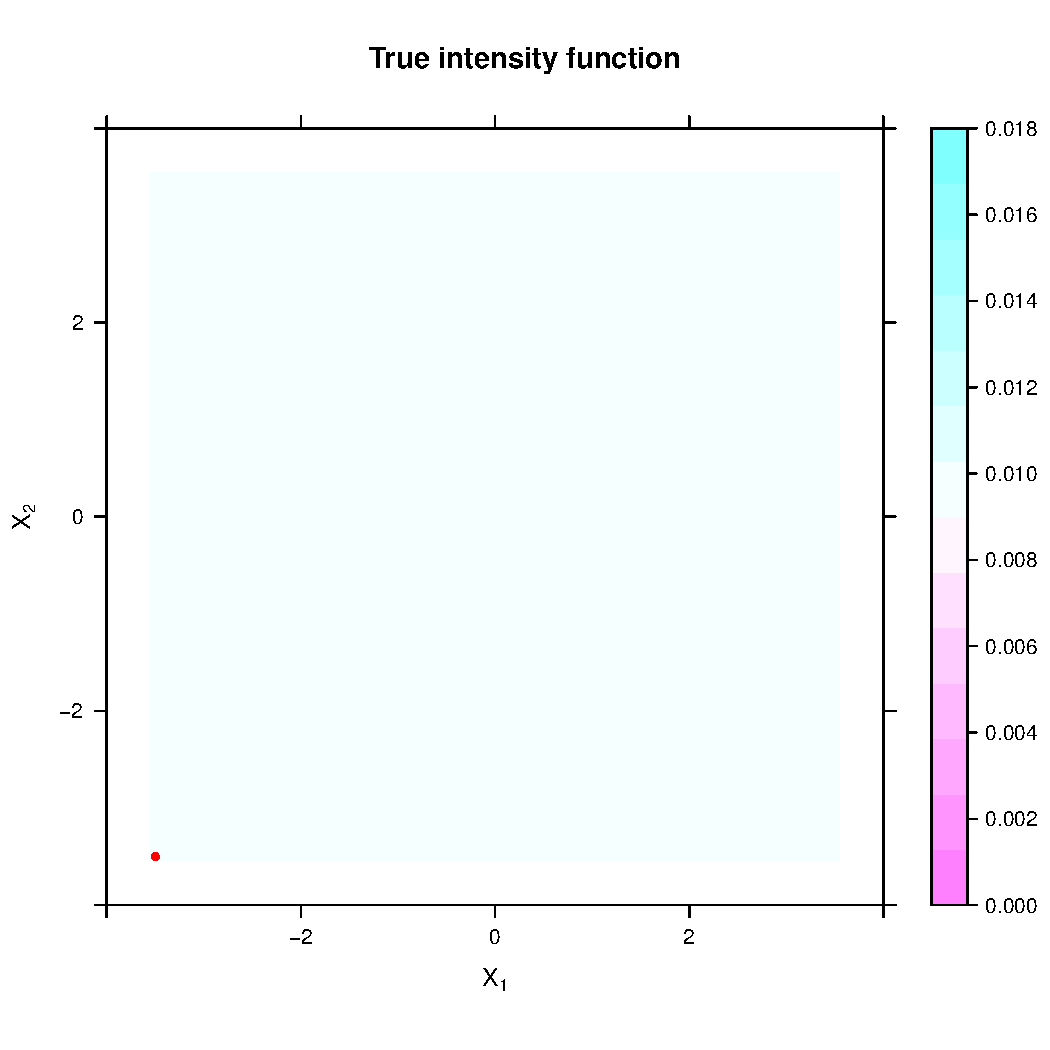
\includegraphics[width=\textwidth]{results/unif_100_unif/output/true_intensity_heatmap}
    \caption{True intensity}
    \end{subfigure}%
    \begin{subfigure}[t]{0.45\textwidth}
    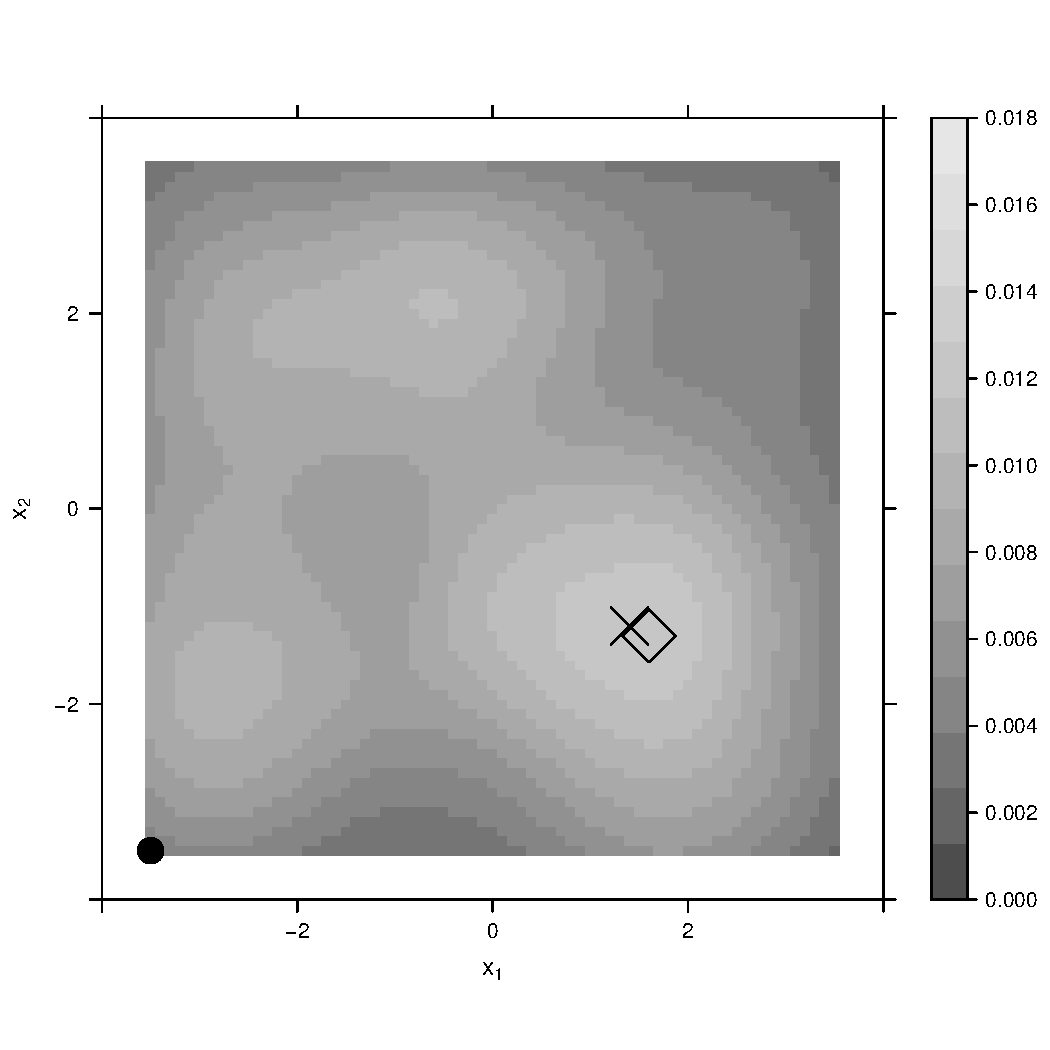
\includegraphics[width=\textwidth]{results/unif_100_unif/output/oracle_intensity_heatmap}
    \caption{Oracle bandwidth estimate}
    \end{subfigure}


    \begin{subfigure}[b]{0.45\textwidth}
    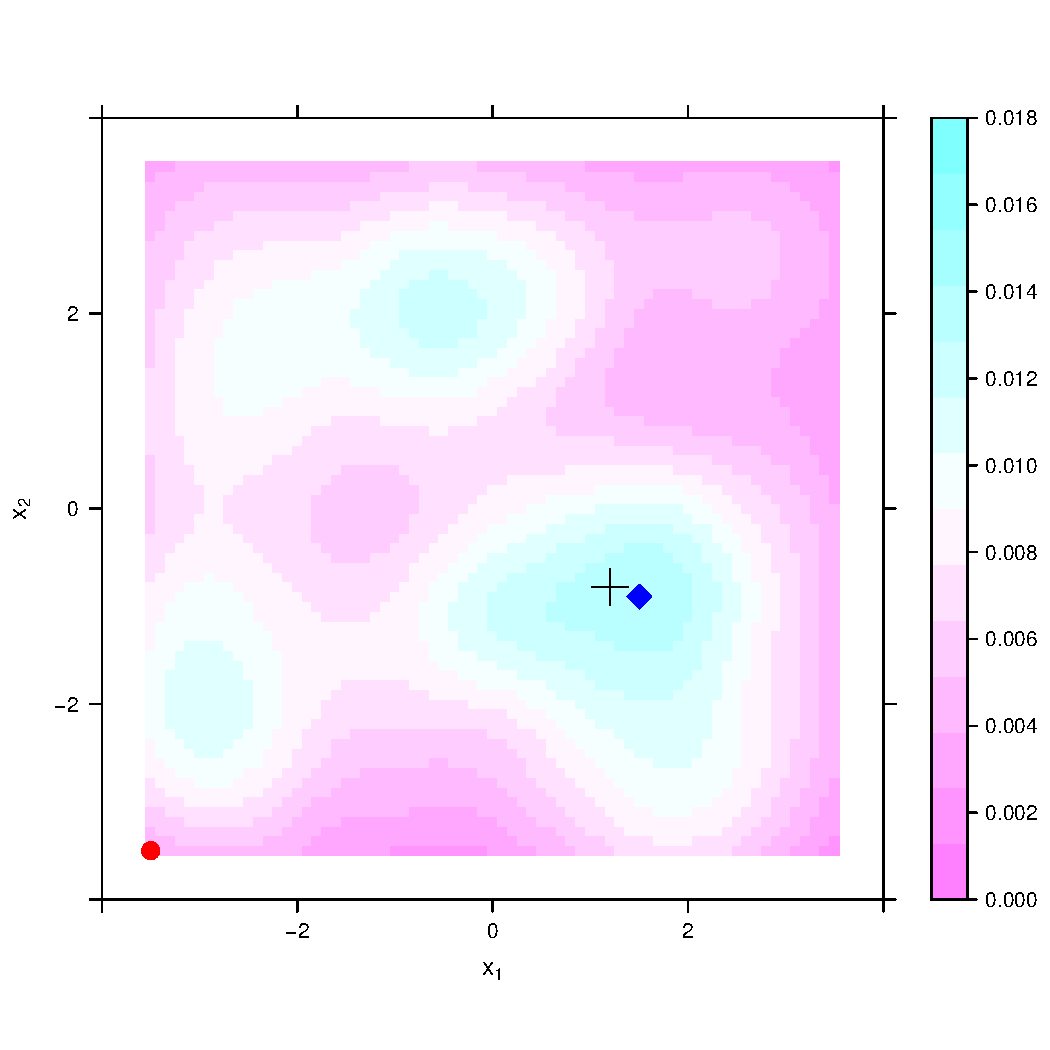
\includegraphics[width=\textwidth]{results/unif_100_unif/output/silverman_intensity_heatmap}
    \caption{Silverman bandwidth estimate}
    \end{subfigure}%
    \begin{subfigure}[b]{0.45\textwidth}
    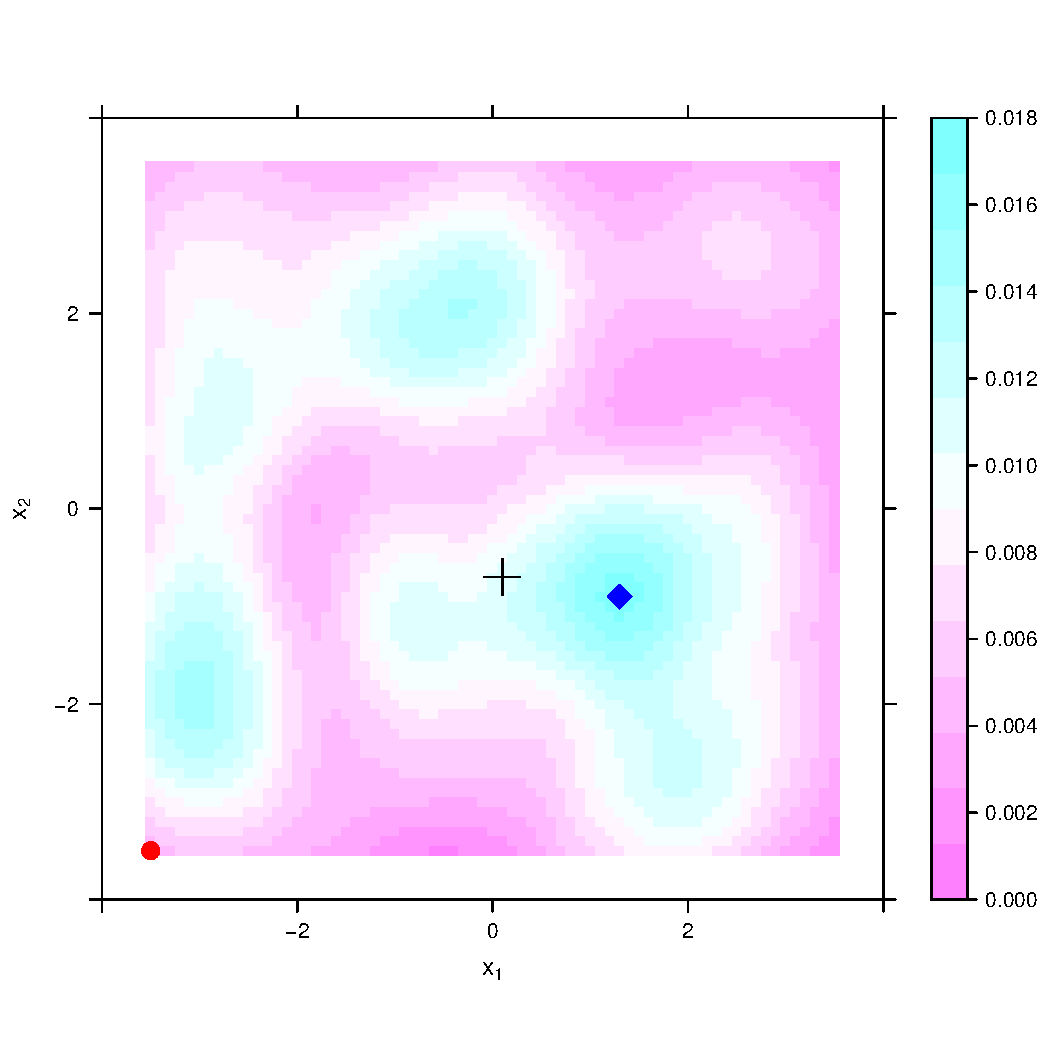
\includegraphics[width=\textwidth]{results/unif_100_unif/output/CV_intensity_heatmap}
    \caption{Cross-validation bandwidth estimate}
    \end{subfigure}
    \caption{Example cases: uniform intensity on uniform population, 100 cases}
    \label{fig:cases:unif_100_unif}
\end{figure}


\autoref{tbl:errors:unif_100_unif} lists the mean error rates obtained for a uniform intensity with factor of 100, over a uniform population of 10,000.
The columns represent the errors observed by using the three different methods for computing the smoothing bandwidth:
the Oracle, the Silverman rule of thumb, and least-squares cross validation.

\begin{figure}[htbp]
    \centering
    \begin{subfigure}[b]{0.45\textwidth}
    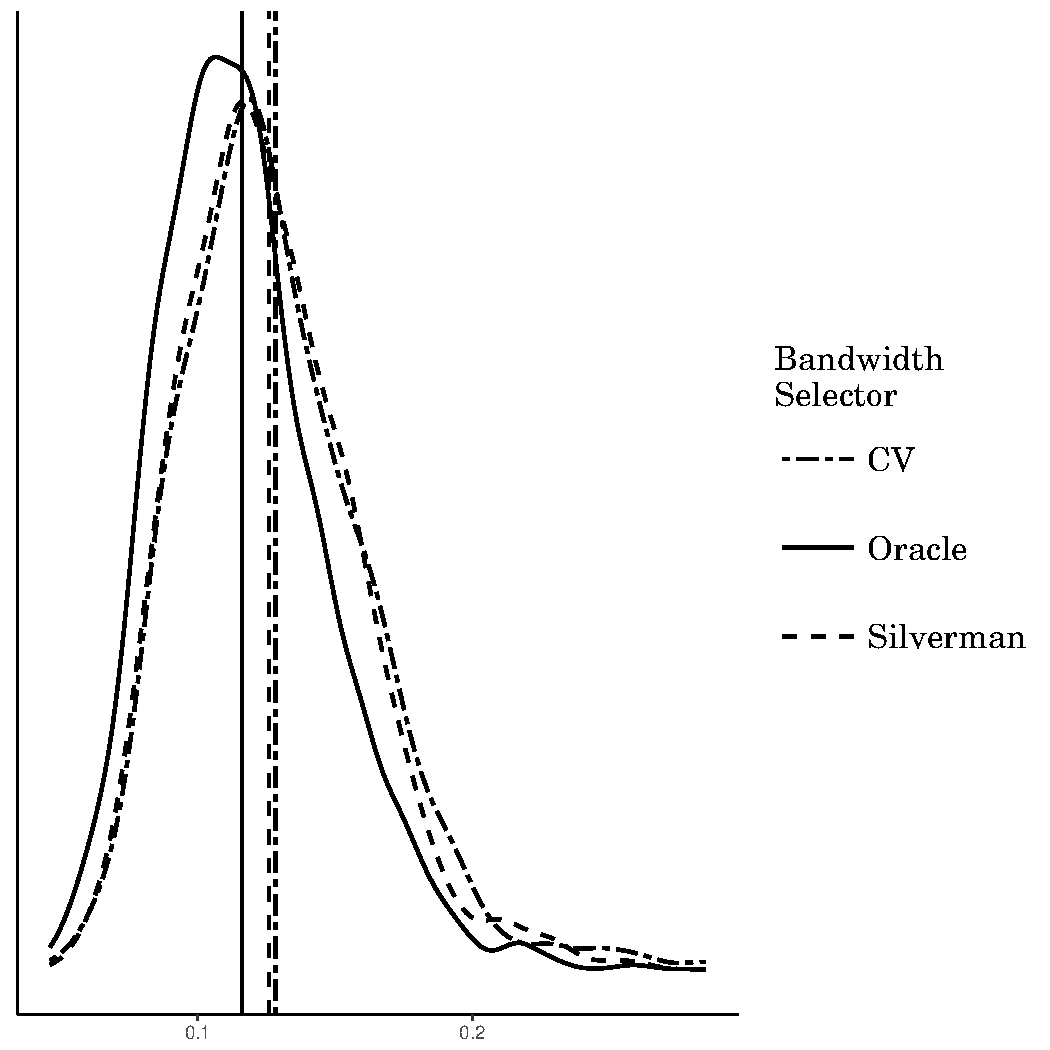
\includegraphics[width=\textwidth]{results/unif_100_unif/output/ise-relative-histogram}
    \caption{Relative ISE}
    \end{subfigure}
    \begin{subfigure}[b]{0.45\textwidth}
    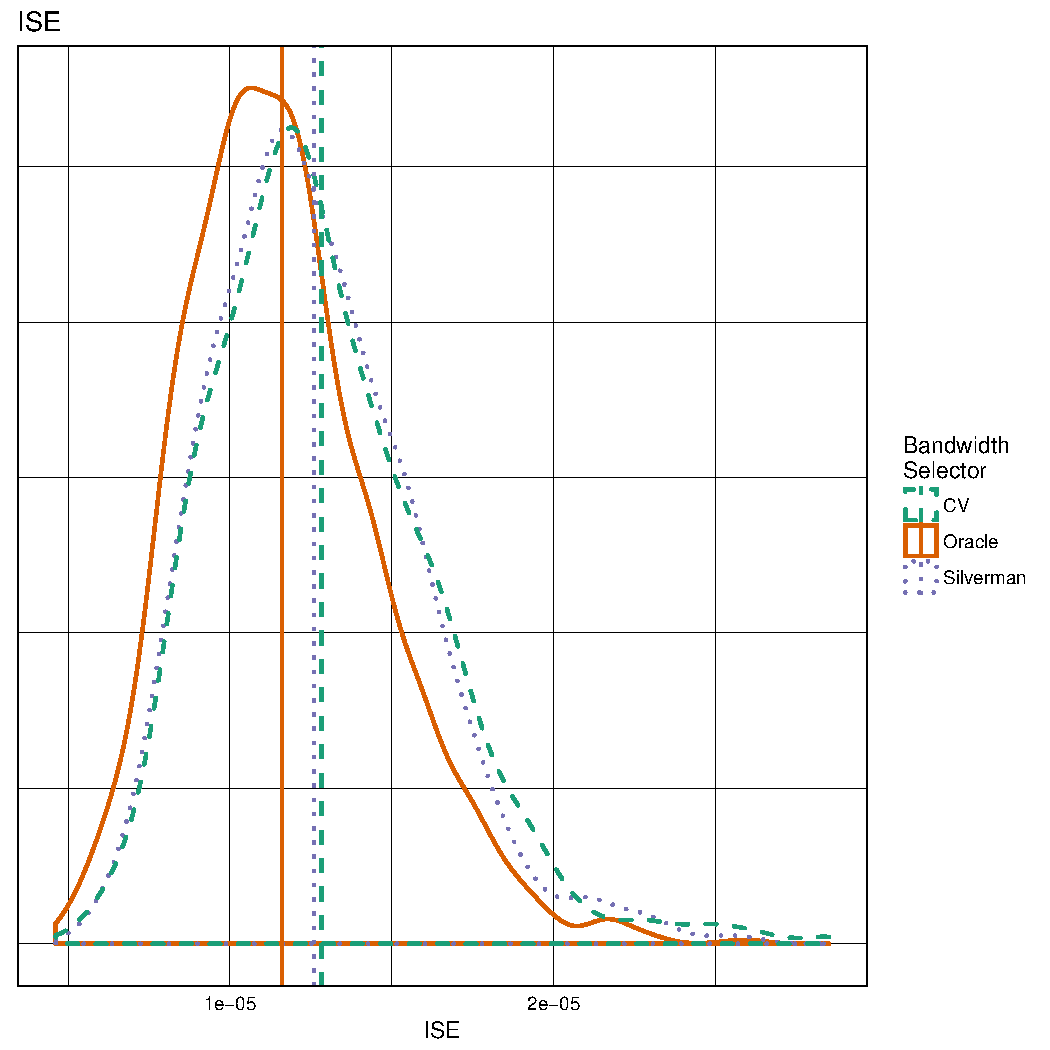
\includegraphics[width=\textwidth]{results/unif_100_unif/output/ise-histogram}
    \caption{Absolute ISE}
    \end{subfigure}
    \caption[ISE: uniform on uniform]{Integrated squared error histogram for uniform intensity on a uniform population, 100 cases}
    \label{fig:ise:unif_100_unif}
\end{figure}

Each row represents a different measure of error.
The first row, MISE, is the mean integrated squared error.
Relative MISE is the mean integrated relative squared error, where the relative squared error is computed in the following manner:
\[ \mbox{RSE}(x) = \left(\frac{\hat{f}(x)-f(x)}{f(x)}\right)^2 .\]
More generally, the relative error at a point \(x\) is computed as
\[ \mbox{RE}(x) =  \frac{\hat{f}(x)-f(x)}{f(x)} .\]
\autoref{fig:ise:unif_100_unif} shows the empirical distribution of the MISE and RMISE for the uniform intensity on uniform population.
The next row is the mean integrated absolute error (MIAE), which is followed by Relative MIAE which is computed analogously to Relative MISE.
This is followed by the Maximum error, which is the greatest absolute error over the study area.
Complete results can be found in \autoref{tbl:mean_error_rates:unif_100_unif} in \autoref{chp:results_tables}.

The error measures mentioned above each compare the closeness of the estimated intensity function to the true funcition.
The following error measures, on the other hand, relate the closeness of the \textit{peak} of the estimate to the true peak.
The \textit{peak bias} is the average difference between the computed and true maxima,
that is the empirical expectation of \(\max{\{\hat{f}(x)\}} - \max{\{f(x)\}}\).
The Relative peak bias is peak bias expressed relative to the true maximum.
The \textit{peak drift} is the Euclidean distance between the estimated peak and the true peak.
The Relative peak drift is the peak drift, expressed relative to the width of the study area.

The next four measures, \textit{centroid bias} and \textit{drift}, and the relative versions of them, are analogous to the peak error measures.
However, instead of comparing the true peak to the peak of the estimate, they compare it to the location and value of the estimate, calculated at the centroid of the top five percent of the estimated function.

\begin{table}[htbp]
\centering
% latex table generated in R 3.4.0 by xtable 1.8-2 package
% Sat Aug  5 20:02:24 2017
\begin{tabular}{lrrr}
  \hline
 & Oracle & Silverman & CV \\ 
  \hline
MISE & 0.000012 & 0.000013 & 0.000013 \\ 
  Relative MISE & 0.117027 & 0.127810 & 0.127803 \\ 
  MIAE & 0.002801 & 0.002922 & 0.002922 \\ 
  Relative MIAE & 0.280127 & 0.292163 & 0.292156 \\ 
  Max Error & 0.008572 & 0.009040 & 0.009040 \\ 
  Peak bias & 0.003361 & 0.005616 & 0.005615 \\ 
  Relative Peak bias & 0.336092 & 0.561583 & 0.561492 \\ 
  Peak drift & 5.163912 & 5.190480 & 5.190393 \\ 
  Relative Peak drift & 0.737702 & 0.741497 & 0.741485 \\ 
  Centroid bias & 0.002819 & 0.003733 & 0.003733 \\ 
  Relative Centroid bias & 0.281890 & 0.373345 & 0.373340 \\ 
  Centroid drift & 5.093476 & 5.086491 & 5.086412 \\ 
  Relative Centroid drift & 0.727639 & 0.726642 & 0.726630 \\ 
   \hline
\end{tabular}

\caption{Mean error rates for uniform population, uniform intensity of factor 100}
\label{tbl:errors:unif_100_unif}
\end{table}

\begin{figure}[htbp]
    \centering
    \begin{subfigure}[b]{0.3\textwidth}
    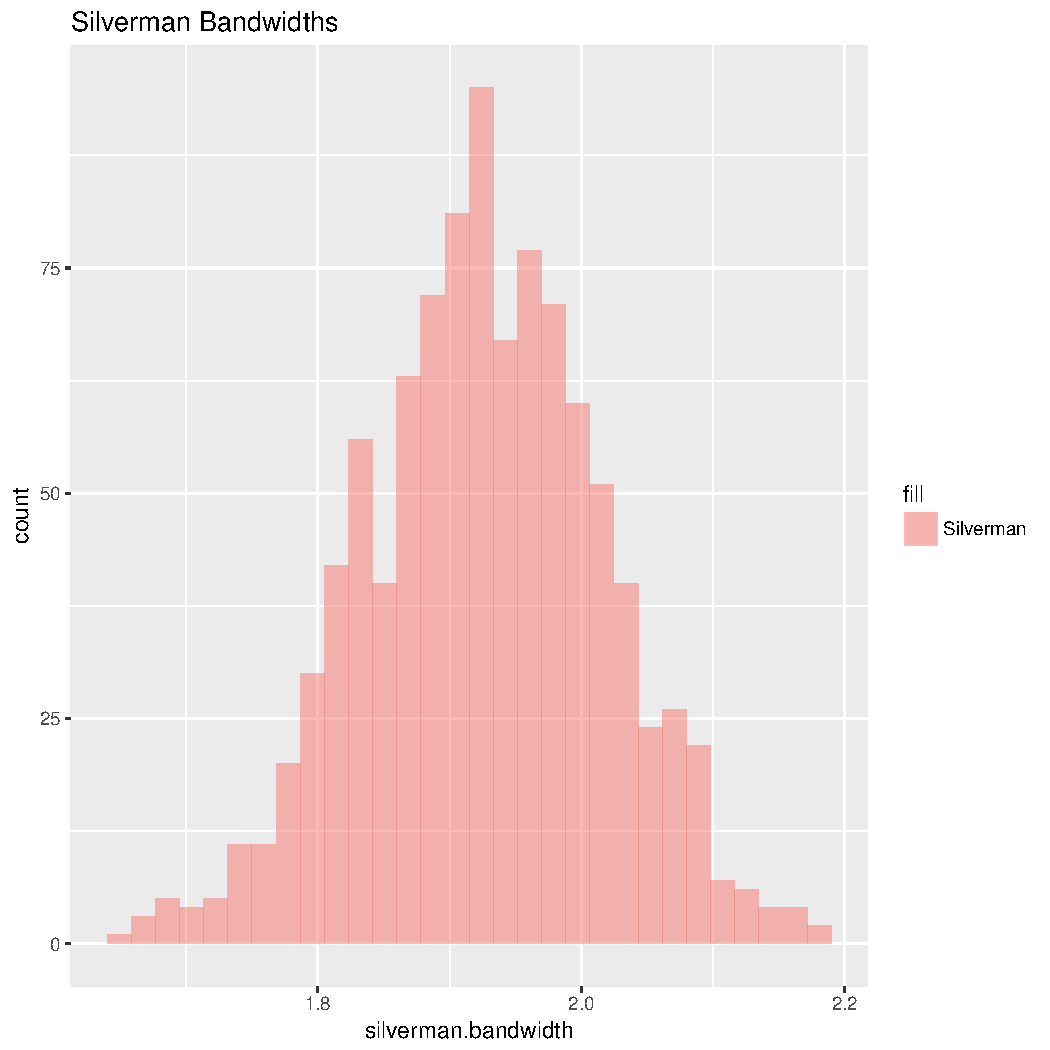
\includegraphics[width=\textwidth]{results/unif_100_unif/output/bandwidths-silverman}
    \caption{Silverman}
    \label{fig:bandwidths_x1:unif_100_unif:s}
    \end{subfigure}
    \begin{subfigure}[b]{0.3\textwidth}
    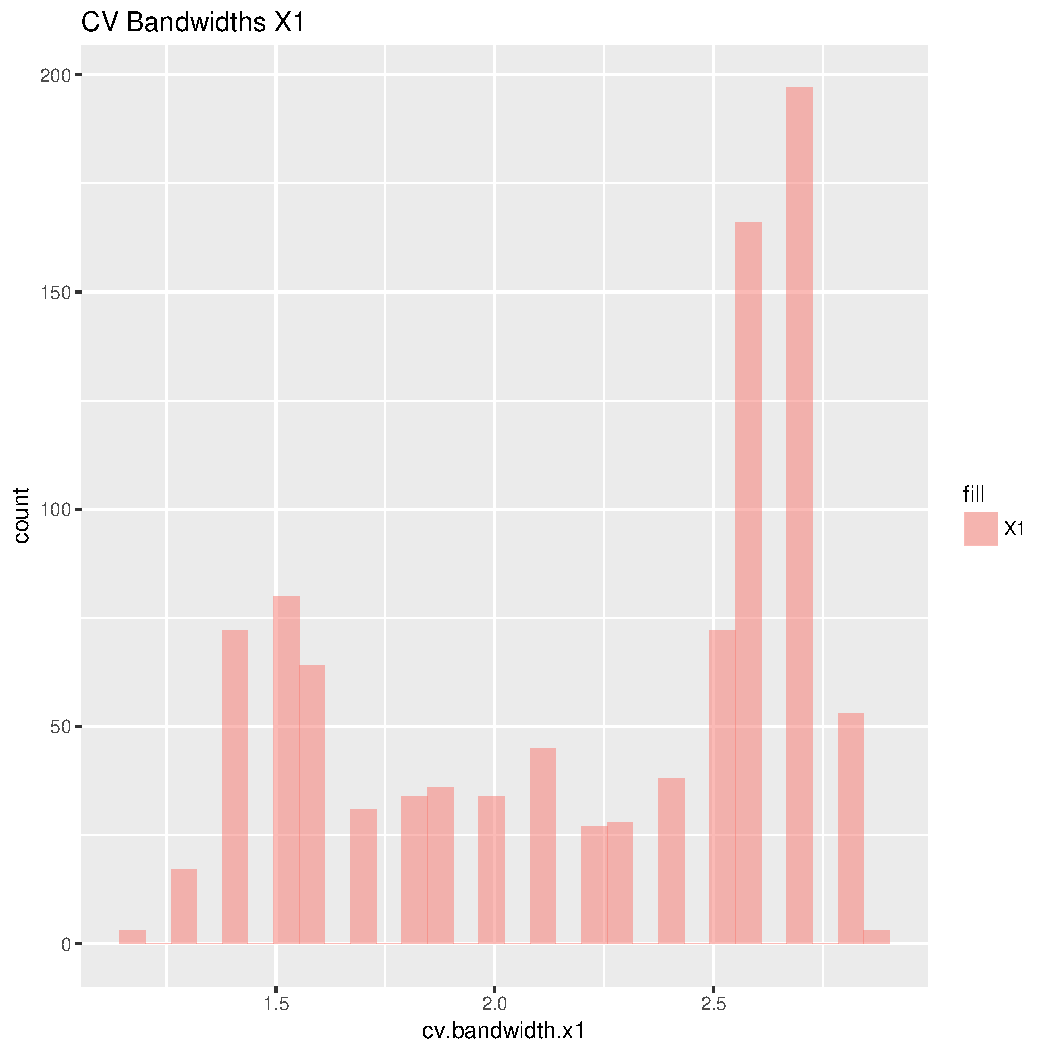
\includegraphics[width=\textwidth]{results/unif_100_unif/output/bandwidths-x1}
    \caption{Cross-validation, \(X_1\)}
    \label{fig:bandwidths_x1:unif_100_unif:x1}
    \end{subfigure}
    \begin{subfigure}[b]{0.3\textwidth}
    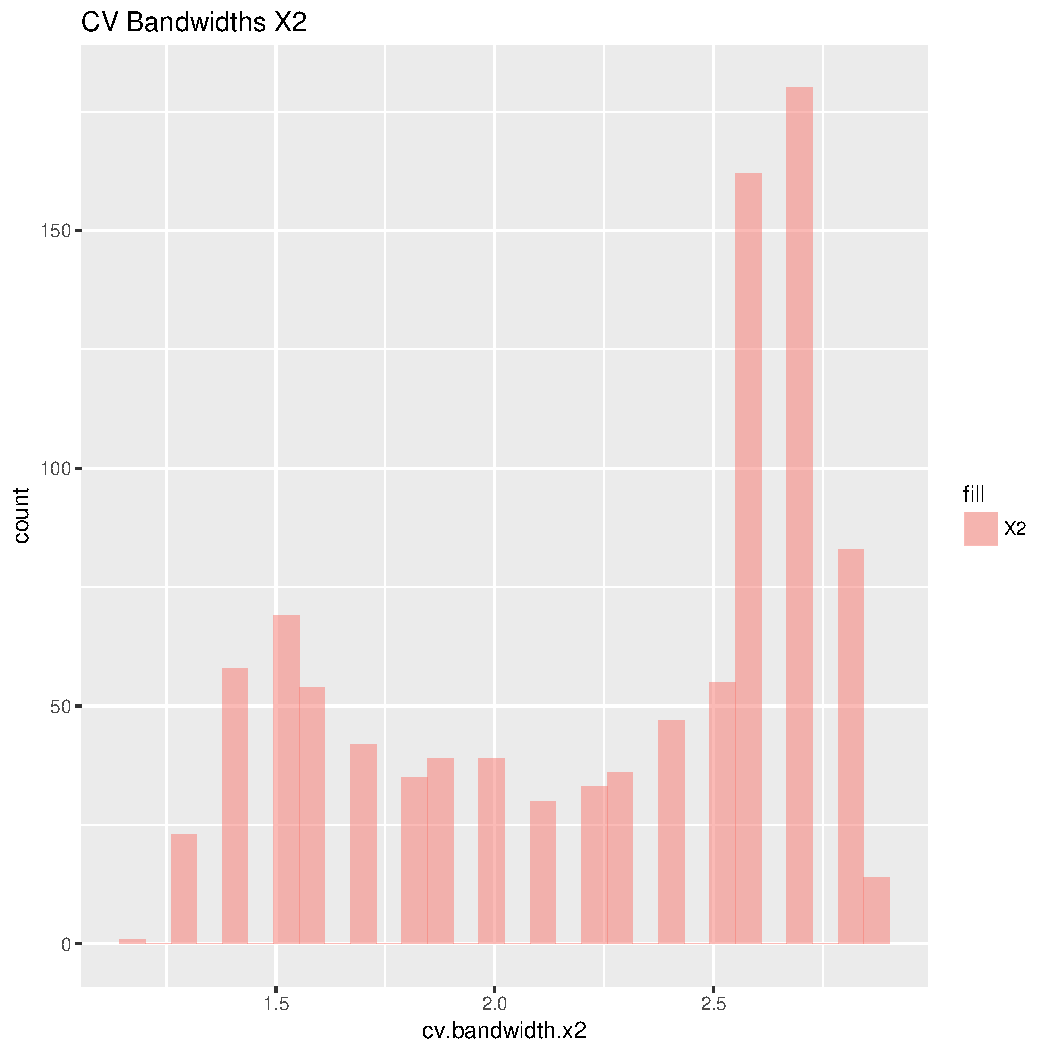
\includegraphics[width=\textwidth]{results/unif_100_unif/output/bandwidths-x2}
    \caption{Cross-validation, \(X_2\)}
    \label{fig:bandwidths_x1:unif_100_unif:x2}
    \end{subfigure}
    \caption{Bandwidth histograms for 100 incidents (uniform) from population of 10,000}
\end{figure}


%%
%% Section
\section{Varying the number of incidents}
\label{sec:results:unif_NCases_1h}

\begin{figure}[htbp]
    \centering
    \begin{subfigure}{0.45\textwidth}
    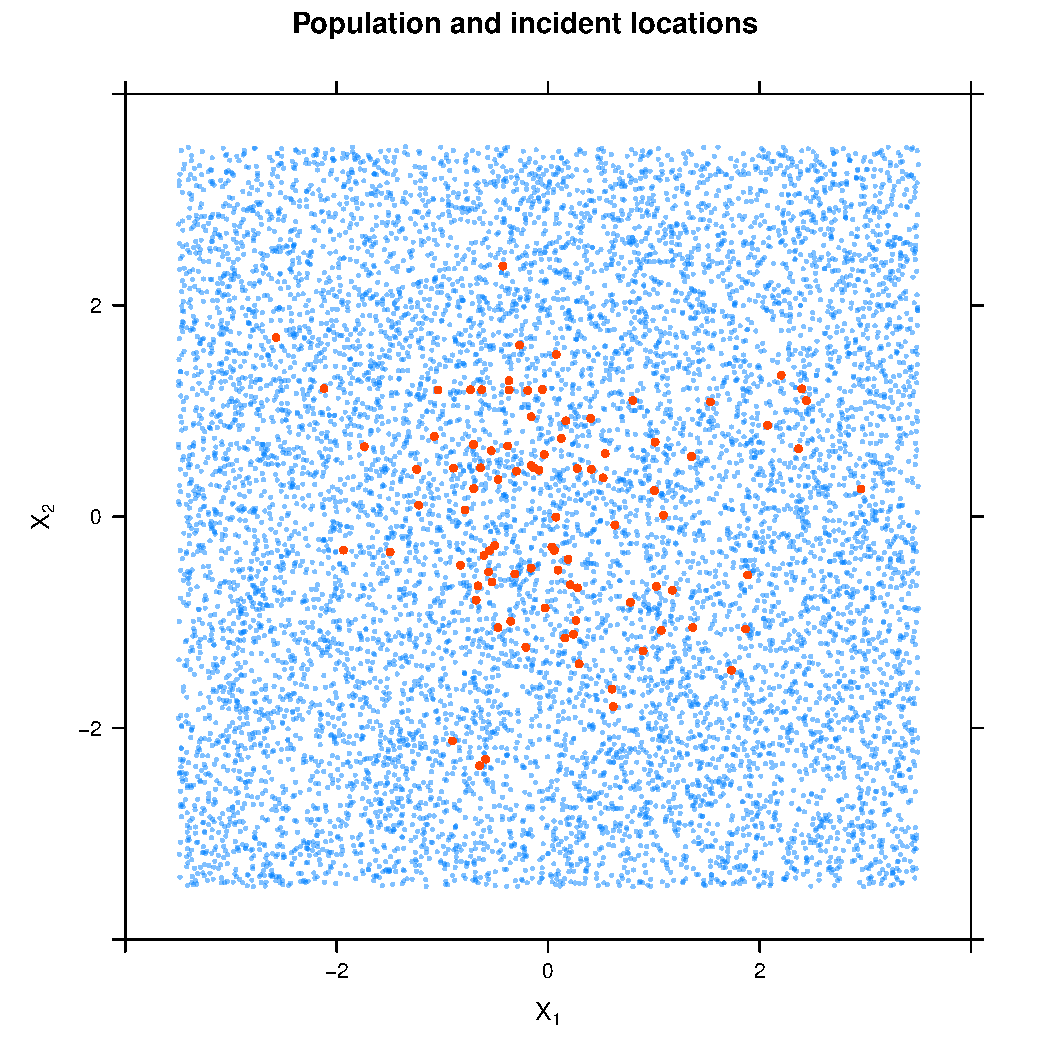
\includegraphics[width=\textwidth]{results/unif_100_1_1h/output/population_and_incidents_scatter}
    \caption{100 incidents}
    \end{subfigure}
    \begin{subfigure}{0.45\textwidth}
    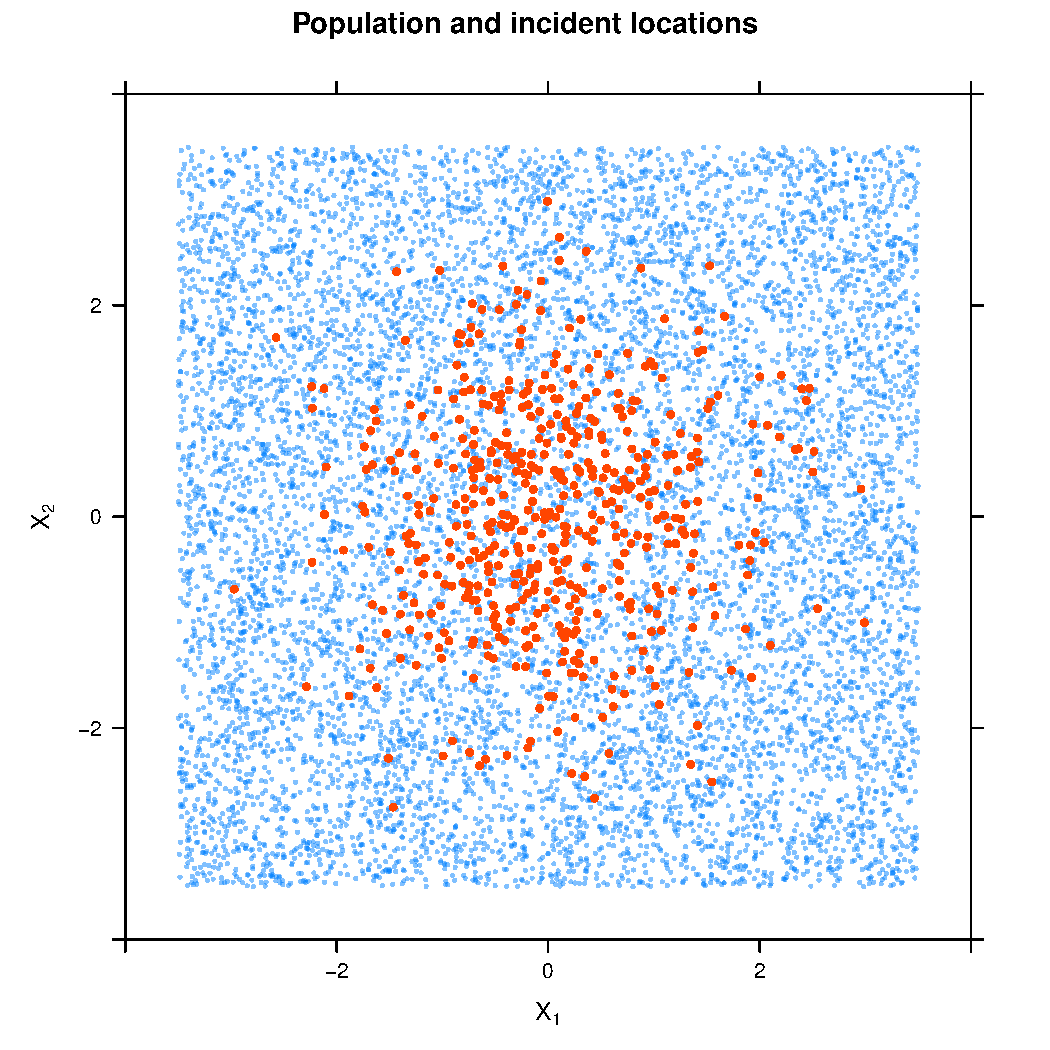
\includegraphics[width=\textwidth]{results/unif_500_1_1h/output/population_and_incidents_scatter}
    \caption{500 incidents}
    \end{subfigure}
    \caption{A single sample of different sizes from a single-peak risk on a uniform population}
    \label{fig:one_sample:unif_NCases_1h}
\end{figure}


\begin{figure}[htbp]
    \centering
    \begin{subfigure}[b]{0.3\textwidth}
    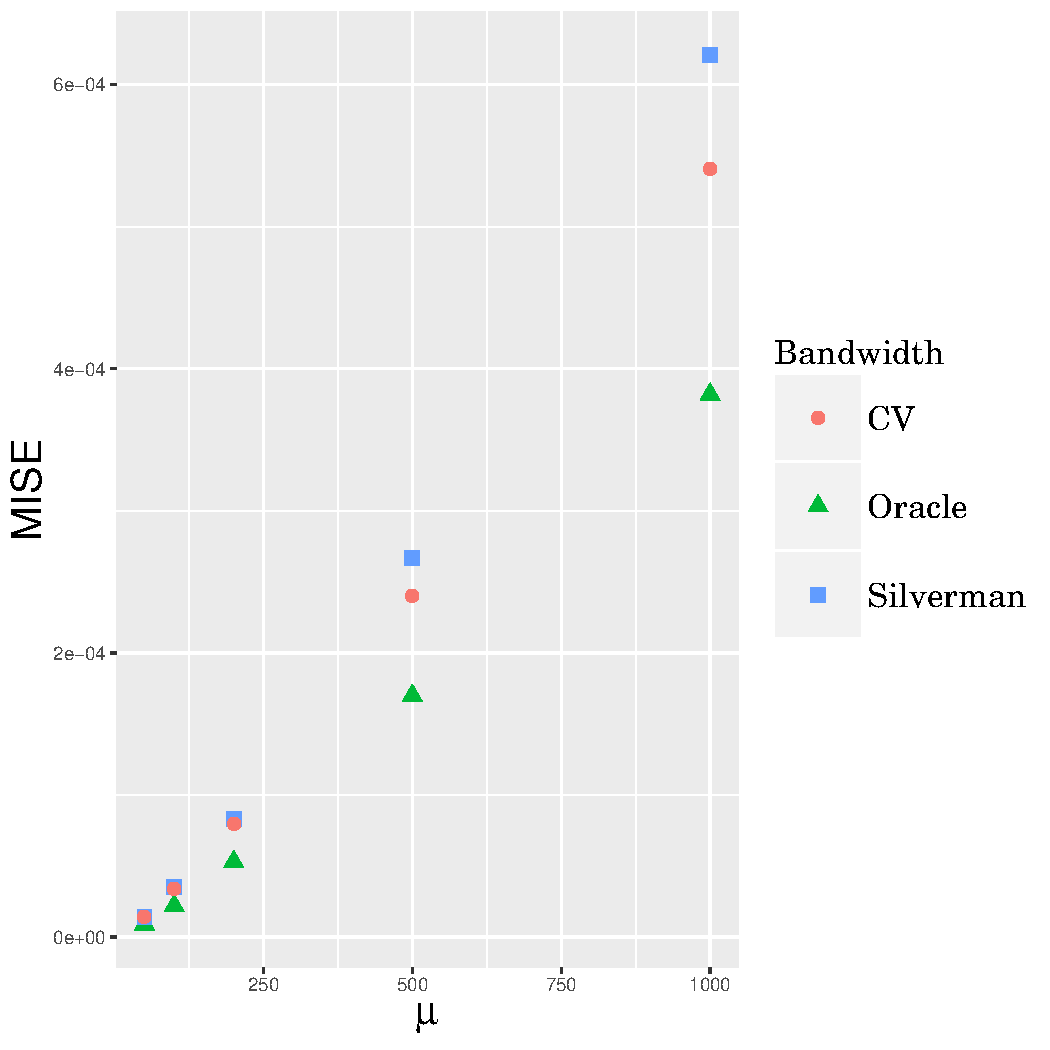
\includegraphics[width=\textwidth]{results/by_num_cases/MISE-vs-cases}
    \caption{MISE}
    \label{fig:ise:unif_NCases_1h:a}
    \end{subfigure}
    \begin{subfigure}[b]{0.3\textwidth}
    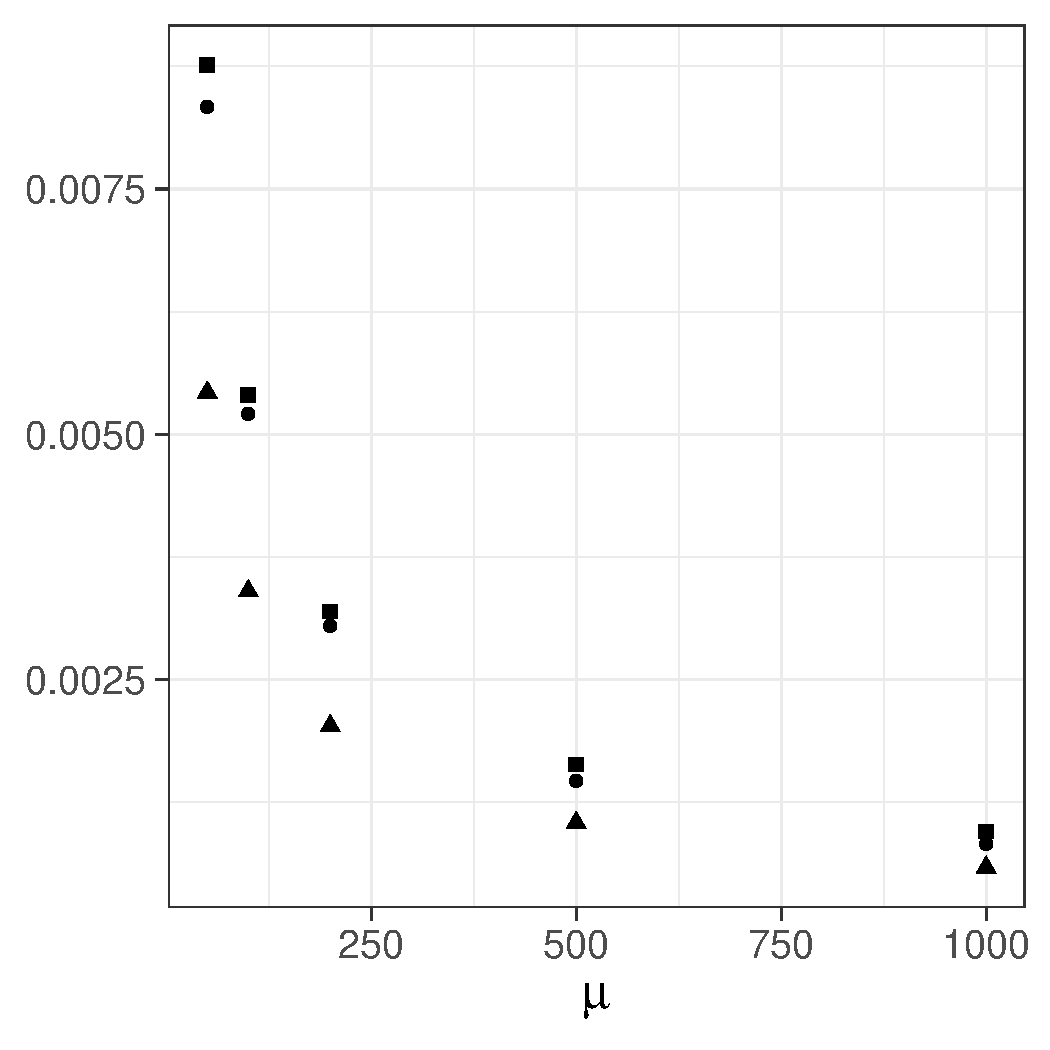
\includegraphics[width=\textwidth]{results/by_num_cases/RMISE-vs-cases}
    \caption{Relative MISE}
    \label{fig:ise:unif_NCases_1h:b}
    \end{subfigure}
    \begin{subfigure}[b]{0.3\textwidth}
    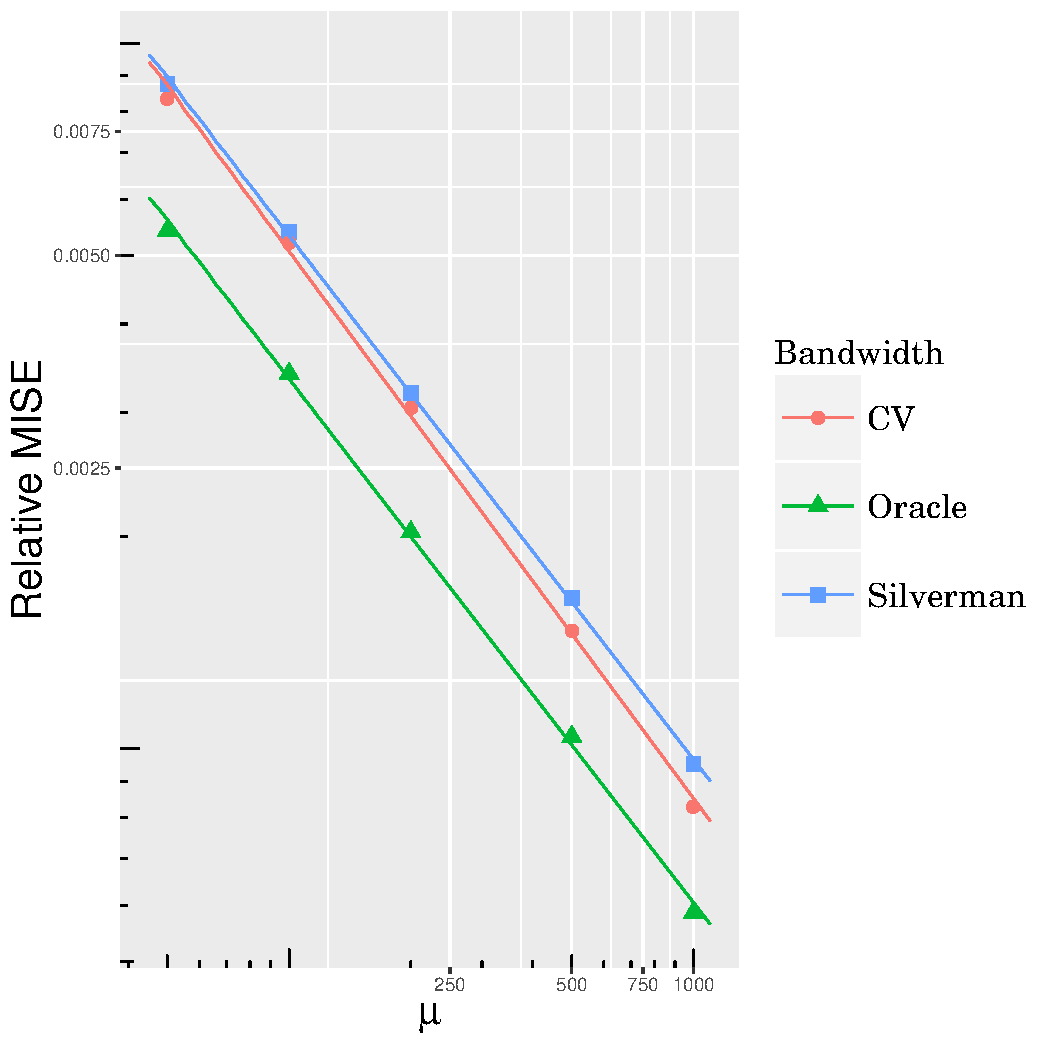
\includegraphics[width=\textwidth]{results/by_num_cases/RMISE-vs-cases-log-log}
    \caption{Relative MISE log-log}
    \label{fig:ise:unif_NCases_1h:c}
    \end{subfigure}
    \caption[MISE: by number of cases]{Mean Integrated Squared Error vs. number of cases}
    \label{fig:ise:unif_NCases_1h}
\end{figure}

In this section we examine and compare the results of experiments where the number of incidents is varied, while keeping the population size constant at 10,000, distributed uniformly throughout the study area.
Sample used in this section were 50, 100, 200, 500, and 1,000.
The full set of error measures for these cases can be found in \autoref{tbl:mean_error_rates:unif_50_1_1h}, \autoref{tbl:mean_error_rates:unif_100_1_1h}, \autoref{tbl:mean_error_rates:unif_200_1_1h}, \autoref{tbl:mean_error_rates:unif_500_1_1h}, and \autoref{tbl:mean_error_rates:unif_100_1_1h} in \autoref{chp:results_tables}.

\begin{figure}[htbp]
    \centering
    \begin{subfigure}[b]{0.3\textwidth}
    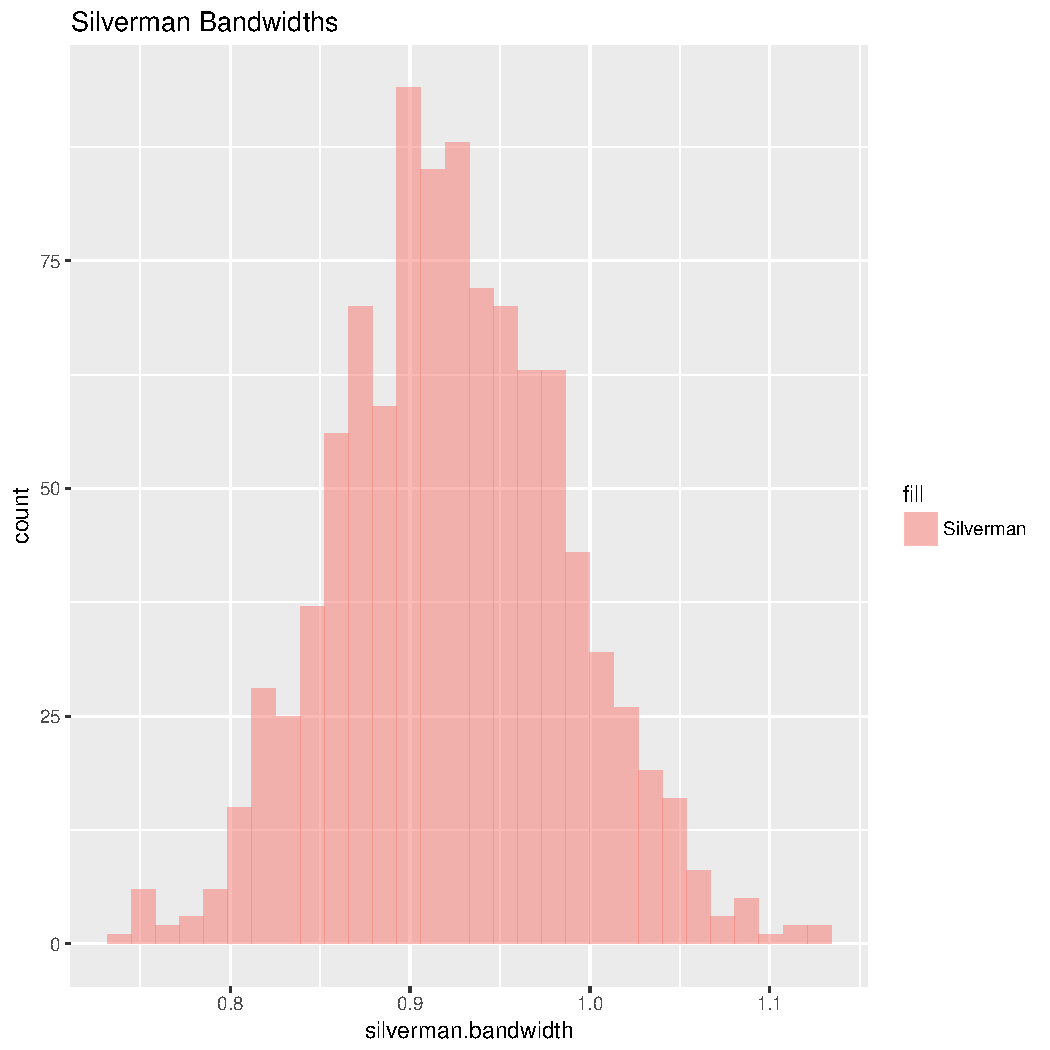
\includegraphics[width=\textwidth]{results/unif_100_1_1h/output/bandwidths-silverman}
    \caption{Silverman}
    \label{fig:bandwidths_x1:unif_100_1_1h:s}
    \end{subfigure}
    \begin{subfigure}[b]{0.3\textwidth}
    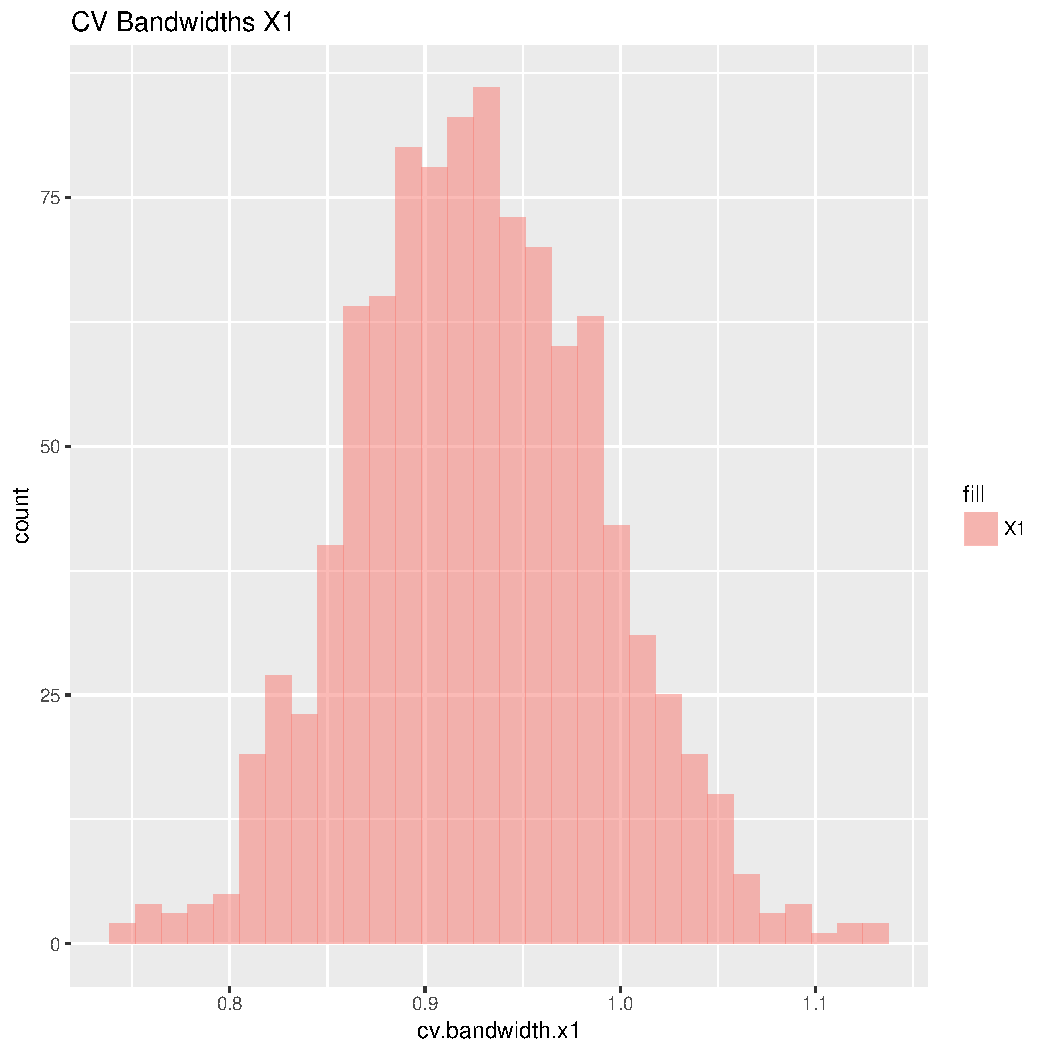
\includegraphics[width=\textwidth]{results/unif_100_1_1h/output/bandwidths-x1}
    \caption{Cross-validation, \(X_1\)}
    \label{fig:bandwidths_x1:unif_100_1_1h:x1}
    \end{subfigure}
    \begin{subfigure}[b]{0.3\textwidth}
    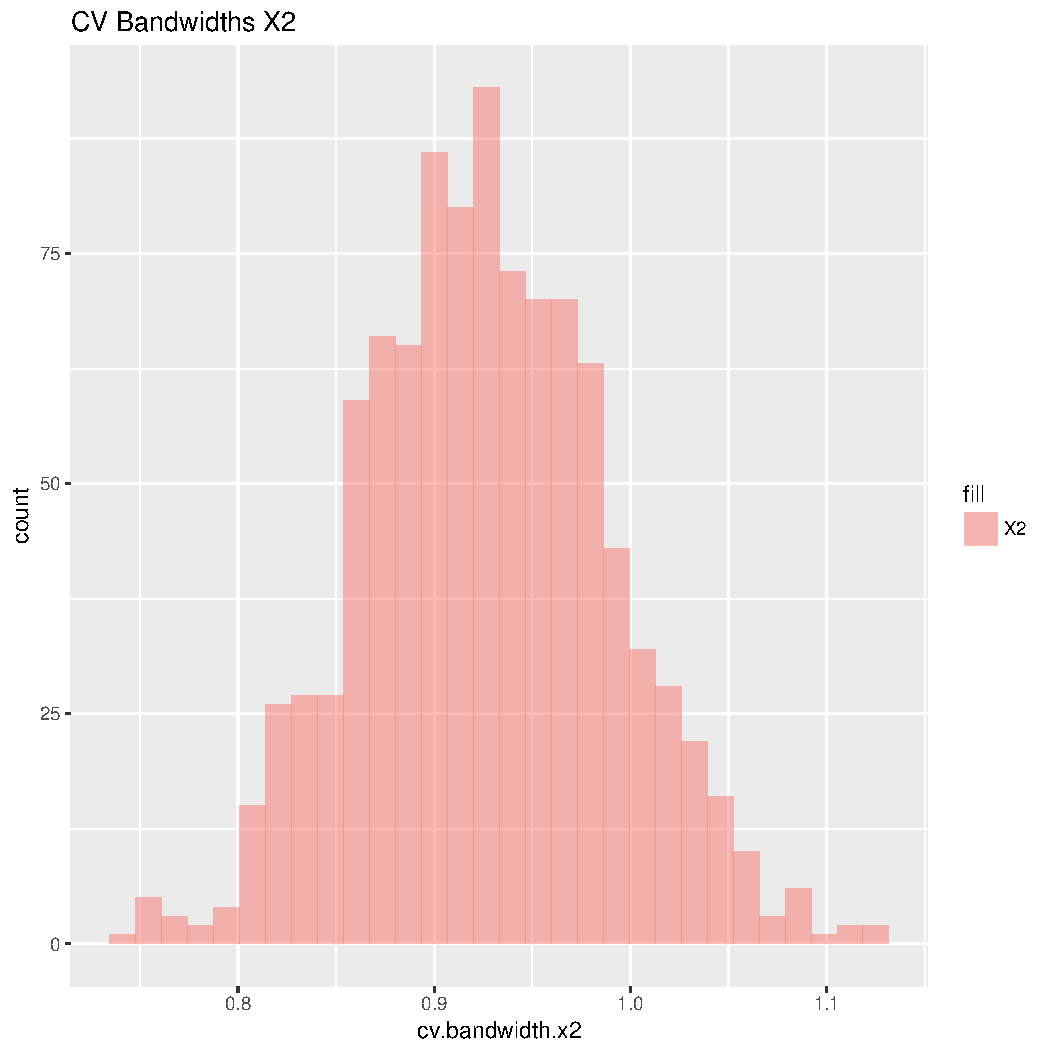
\includegraphics[width=\textwidth]{results/unif_100_1_1h/output/bandwidths-x2}
    \caption{Cross-validation, \(X_2\)}
    \label{fig:bandwidths_x1:unif_100_1_1h:x2}
    \end{subfigure}
    \caption{Bandwidth histograms for 100 incidents in a single peak from population of 10,000}
\end{figure}

\autoref{fig:one_sample:unif_NCases_1h} shows how one sample of incidents, distributed over the population, for sample sizes of 100 and 500.
This is done by multiplying the single-peak risk function by a constant in order to control the expected number of incidents per simulation.
\autoref{fig:ise:unif_NCases_1h} shows the effect on the MISE and RMISE:
\autoref{fig:ise:unif_NCases_1h:a} shows how MISE increases with expected incidents per patient.
One might expect the error to associated with estimating a function to \textit{decrease} as the number of incidents increases.
However, the expected number of incidents increases linearly with the intensity function value.
For example, double the number of incidents corresponds to an intensity of twice the value.
This makes comparing the MISE of estimates of intensity functions difficult, as the errors will also rise in the same direction.
In order to facilitate the comparison of intensity functions that have different expected number of incidents, we use the RMISE.
\autoref{fig:ise:unif_NCases_1h:b} shows how RMISE decreases with expected incidents per patient.
\autoref{fig:ise:unif_NCases_1h:c} is a log-log graph, showing a linear relationship between the logarithm of RMISE and the logarithm of the number of cases.
The values of the intercept and slope are -2.3525396 and -0.7316768 for the Oracle bandwidth; -1.8623772 and -0.7356884 for the Silverman bandwidth; and -1.5308541 and -0.8103349 for the cross-validation bandwidth.
The corresponding equations for RMISE are:

\begin{align}
    \mbox{RMISE}_{oracle} &= 0.09512727 N^{-0.7316768} \\
    \mbox{RMISE}_{silverman} &= 0.155303 N^{-0.7356884} \\
    \mbox{RMISE}_{cv} &= 0.2163508 N^{-0.8103349}
\end{align}



%%
%% Section
\section{Varying the size of the population}
\label{sec:results:unifNpop_1h}

\begin{figure}[htbp]
    \centering
    \begin{subfigure}[b]{0.3\textwidth}
    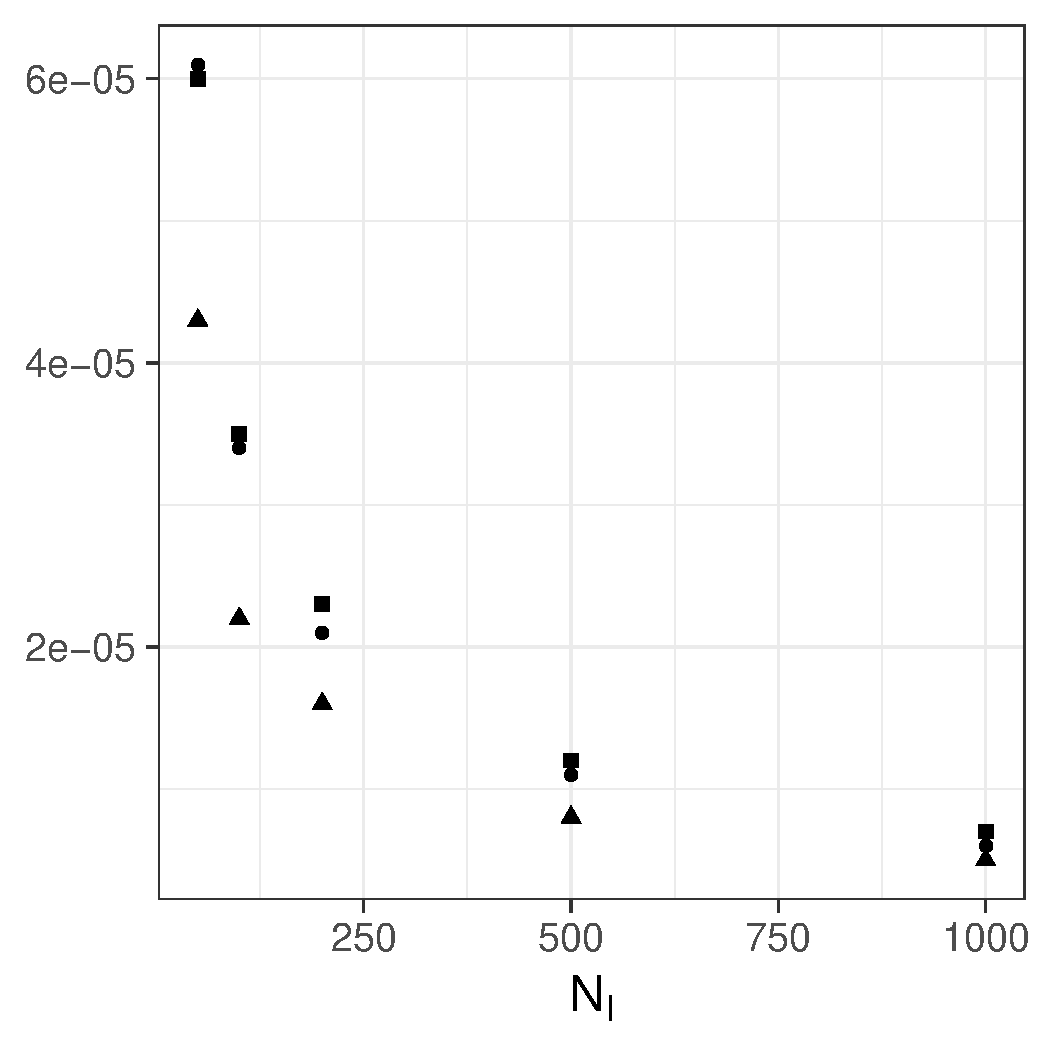
\includegraphics[width=\textwidth]{results/by_pop_size/MISE-vs-population}
    \caption{MISE}
    \end{subfigure}
    \begin{subfigure}[b]{0.3\textwidth}
    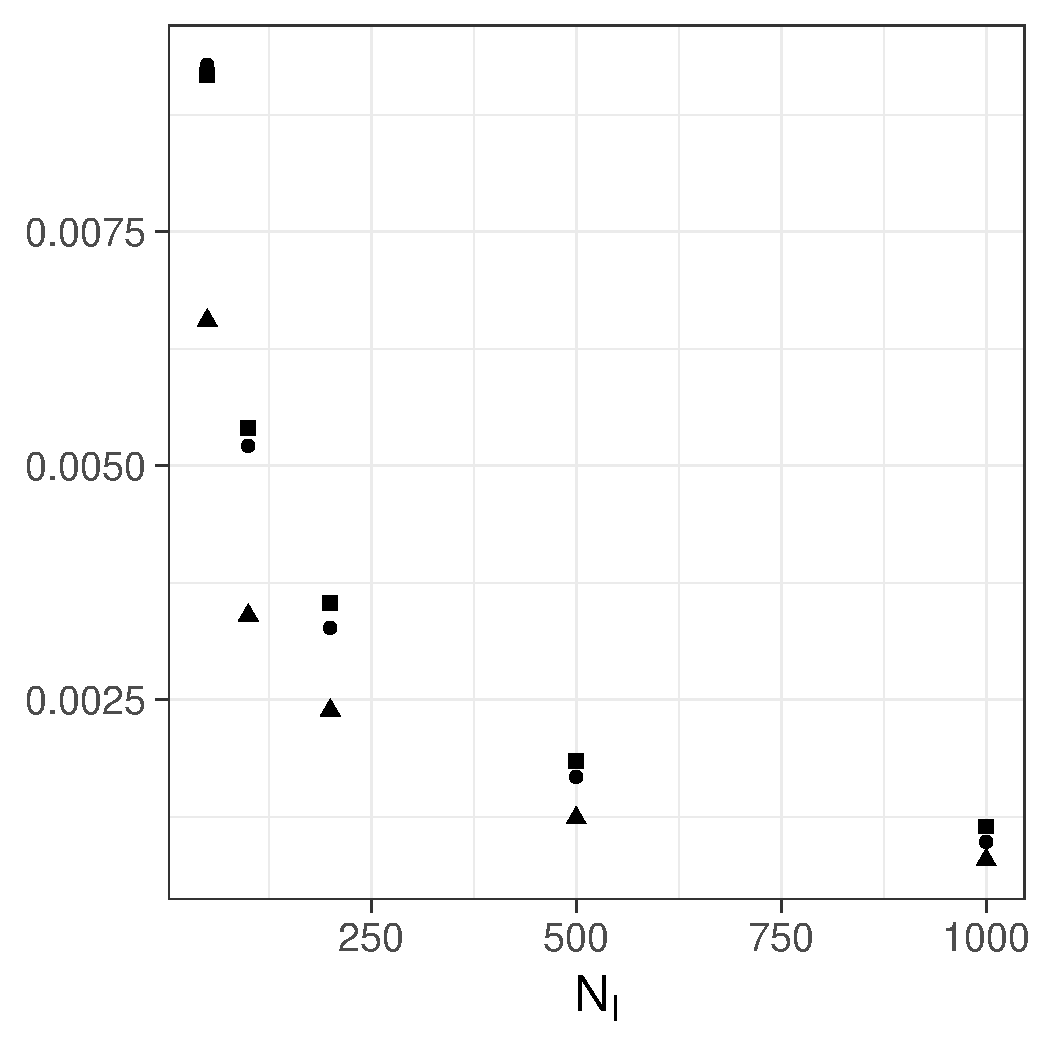
\includegraphics[width=\textwidth]{results/by_pop_size/RMISE-vs-population}
    \caption{Relative MISE}
    \end{subfigure}
    \begin{subfigure}[b]{0.3\textwidth}
    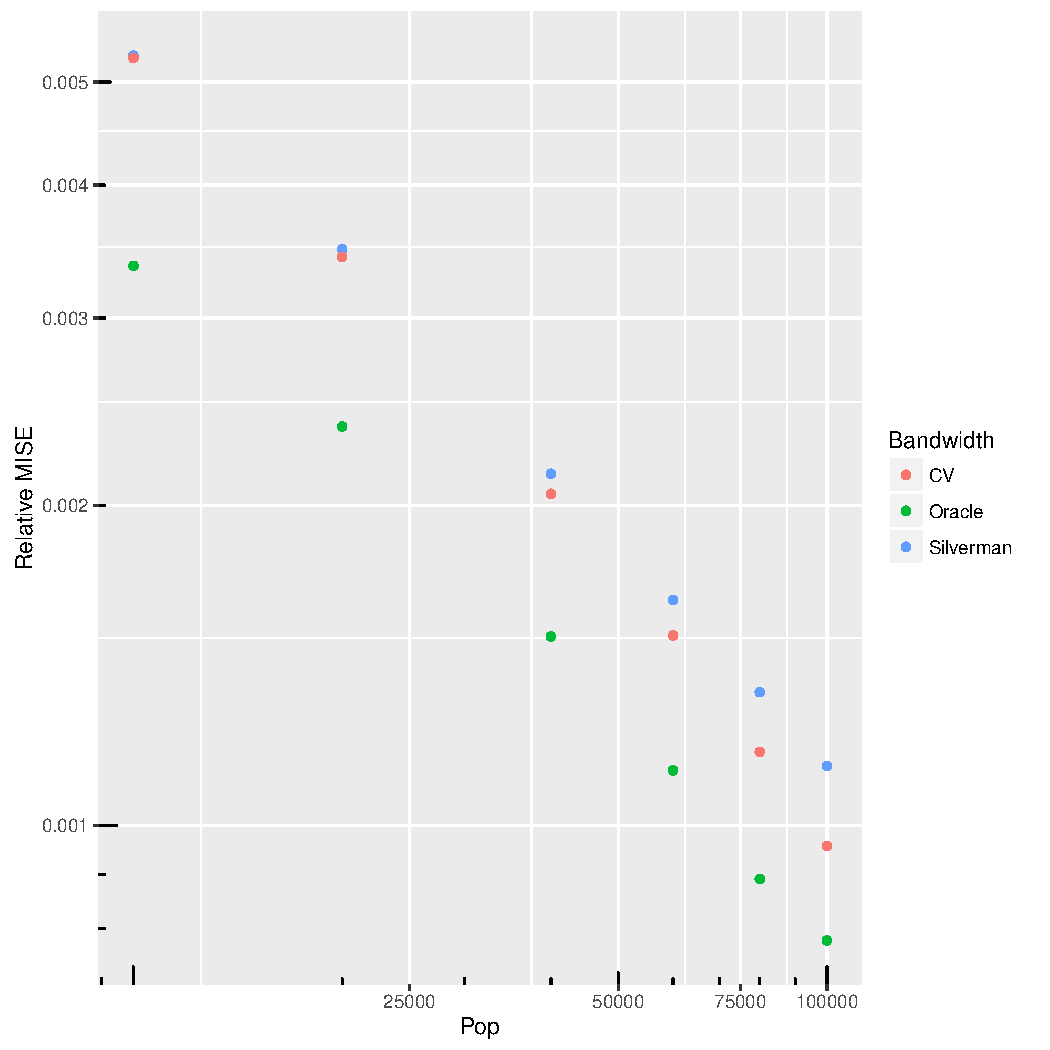
\includegraphics[width=\textwidth]{results/by_pop_size/RMISE-vs-population-log-log}
    \caption{Relative MISE log-log}
    \end{subfigure}
    \caption[MISE: by population size]{Mean Integrated Squared Error vs. population size}
    \label{fig:ise:unifNpop_1h}
\end{figure}


%%
%% Section
\section{Varying the decay of the risk function}
\label{sec:results:unif_100_SD}

\begin{figure}[htbp]
    \centering
    \begin{subfigure}[b]{0.3\textwidth}
    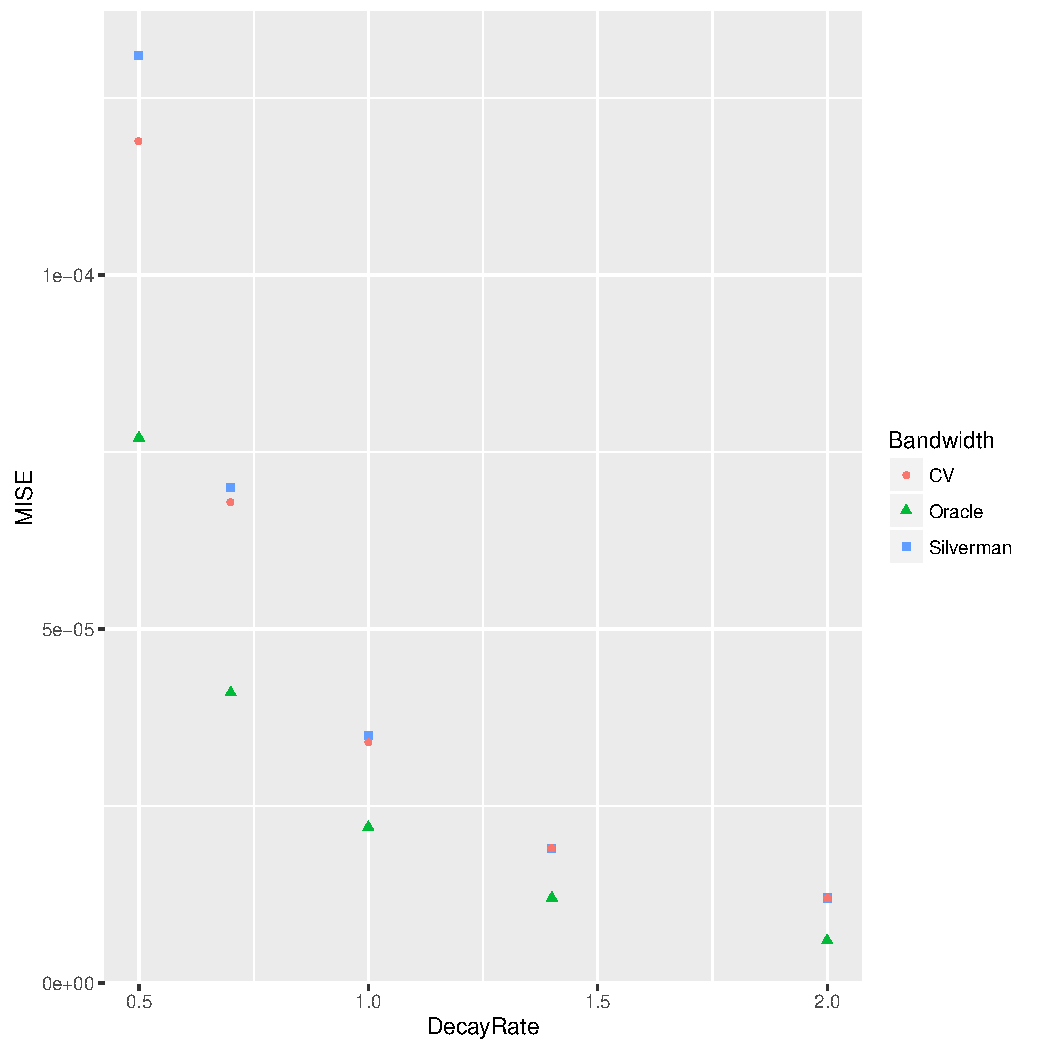
\includegraphics[width=\textwidth]{results/by_cases_decay/MISE-vs-risk-decay}
    \caption{MISE}
    \end{subfigure}
    \begin{subfigure}[b]{0.3\textwidth}
    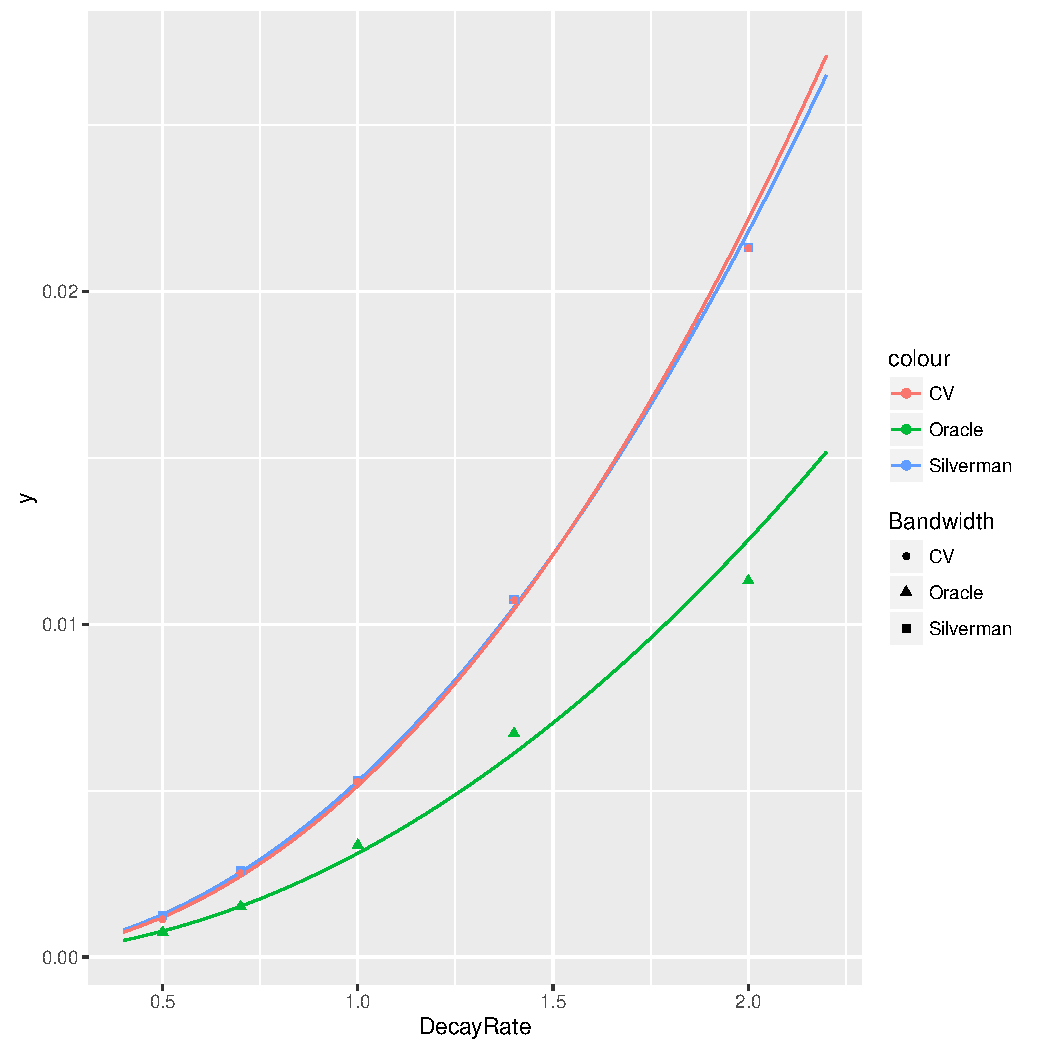
\includegraphics[width=\textwidth]{results/by_cases_decay/RMISE-vs-risk-decay}
    \caption{Relative MISE}
    \end{subfigure}
    \begin{subfigure}[b]{0.3\textwidth}
    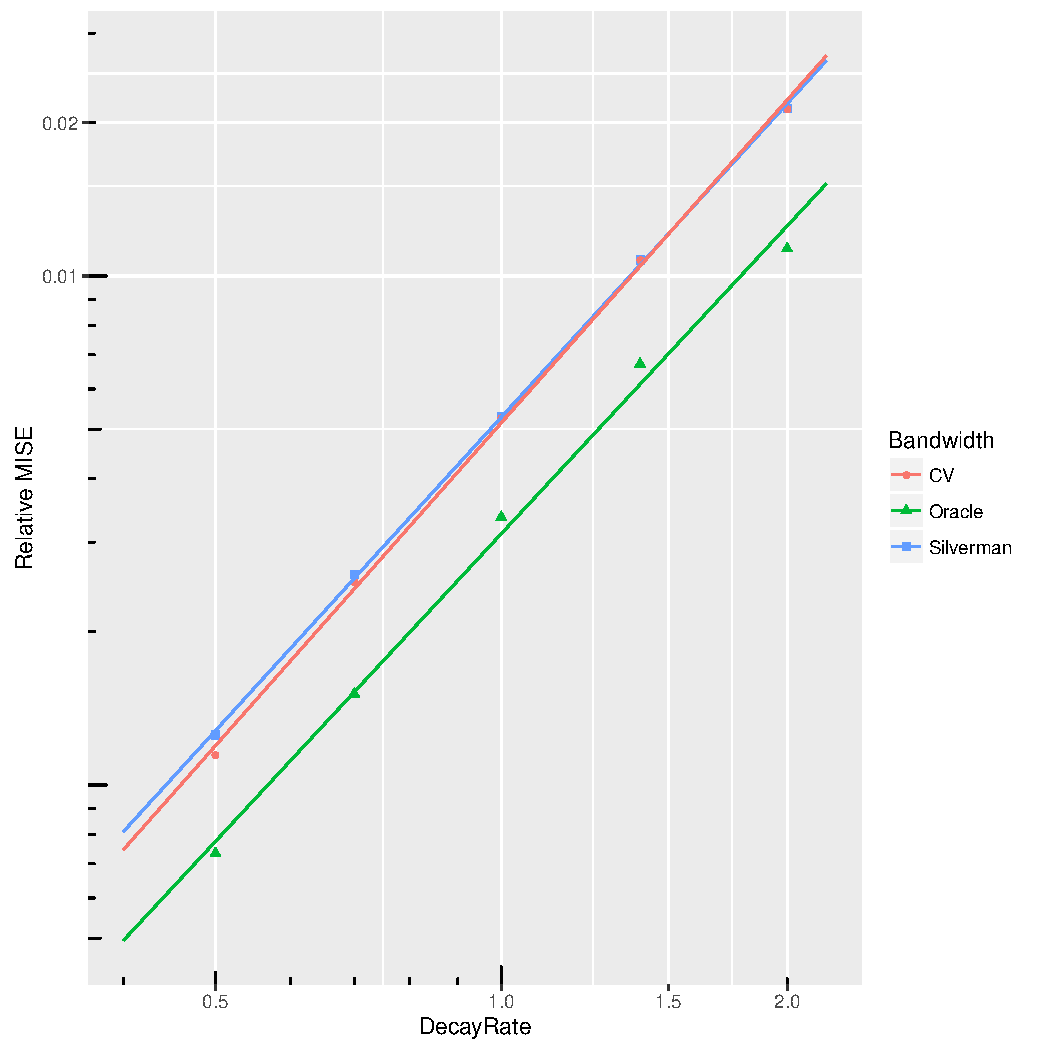
\includegraphics[width=\textwidth]{results/by_cases_decay/RMISE-vs-risk-decay-log-log}
    \caption{Relative MISE log-log}
    \end{subfigure}
    \caption[MISE: by risk decay]{Mean Integrated Squared Error vs. risk decay rate}
    \label{fig:ise:unif_100_SD}
\end{figure}

%%
%% Section
\section{Varying the decay of the population density}
\label{sec:results:pSD_100_1h}

\begin{table}[htbp]
\centering
% latex table generated in R 3.4.0 by xtable 1.8-2 package
% Sat Aug  5 23:40:16 2017
\begin{table}[H]
\centering
\begin{tabular}{lrrr}
  \hline
 & Oracle & Silverman & CV \\ 
  \hline
MISE & 0.001551 & 0.001488 & 13455866197.588720 \\ 
  Relative MISE & 0.237723 & 0.227961 & 2062001845964.798828 \\ 
  MIAE & 0.006198 & 0.006264 & 516.211152 \\ 
  Relative MIAE & 0.076728 & 0.077543 & 6390.223929 \\ 
  Max Error & 0.401935 & 0.425882 & 148124.498061 \\ 
  Peak bias & 0.328253 & 0.352447 & 0.302431 \\ 
  Relative Peak bias & 4.063469 & 4.362974 & 3.743822 \\ 
  Peak drift & 2.208545 & 2.202533 & 2.260982 \\ 
  Relative Peak drift & 0.315506 & 0.314648 & 0.322997 \\ 
  Centroid bias & -0.008139 & -0.006532 & -0.013600 \\ 
  Relative Centroid bias & -0.100757 & -0.080862 & -0.168350 \\ 
  Centroid drift & 0.325652 & 0.299875 & 0.438476 \\ 
  Relative Centroid drift & 0.046522 & 0.042839 & 0.062639 \\ 
   \hline
\end{tabular}
\caption{Mean error rates} 
\label{tbl:mean_error_rates}
\end{table}

\caption{Error rates for uniform population of 10,000, single peak intensity of factor 100 and decay rate 0.7}
\label{tbl:results:p0.7_100_1_1h}
\end{table}


\begin{figure}[htbp]
    \centering
    \begin{subfigure}[b]{0.3\textwidth}
    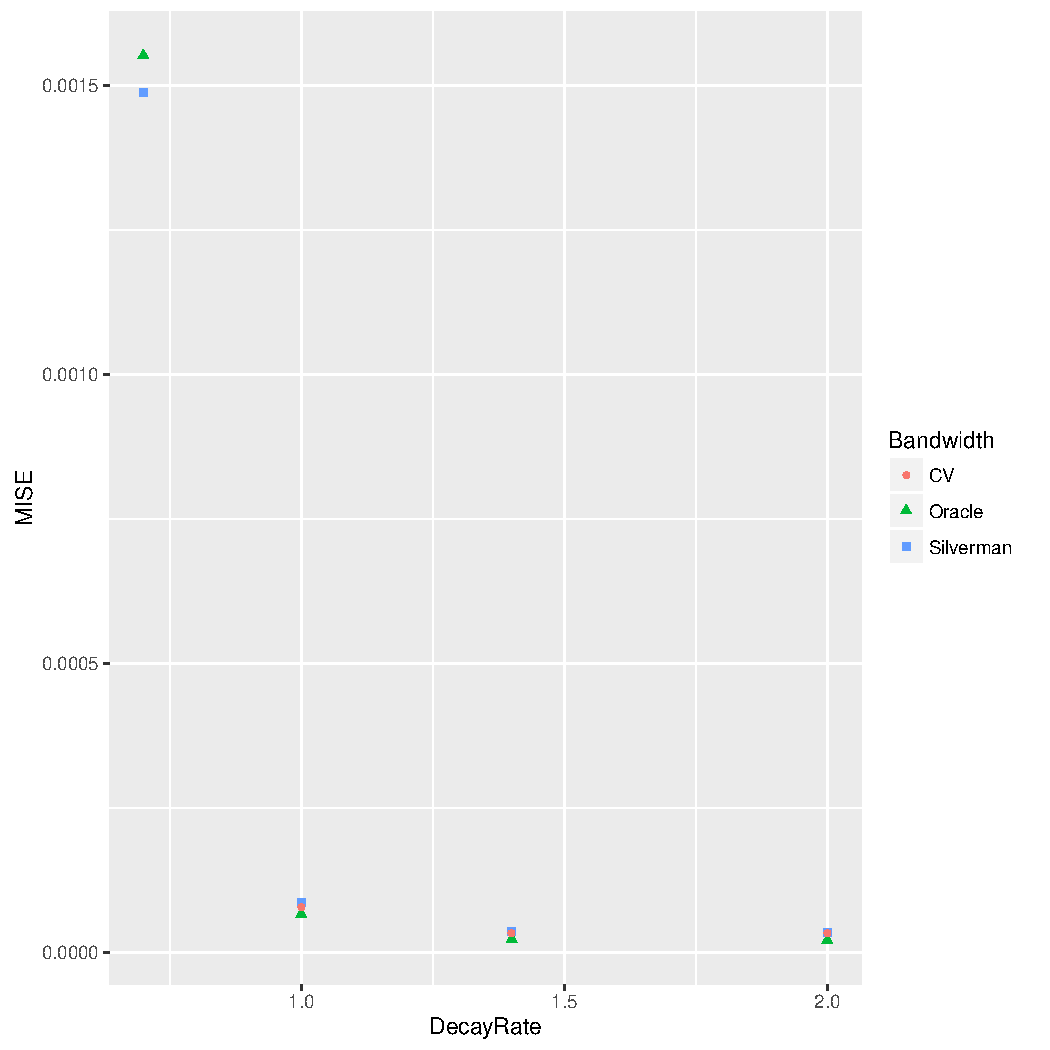
\includegraphics[width=\textwidth]{results/by_population_decay/MISE-vs-population-decay}
    \caption{MISE}
    \end{subfigure}
    \begin{subfigure}[b]{0.3\textwidth}
    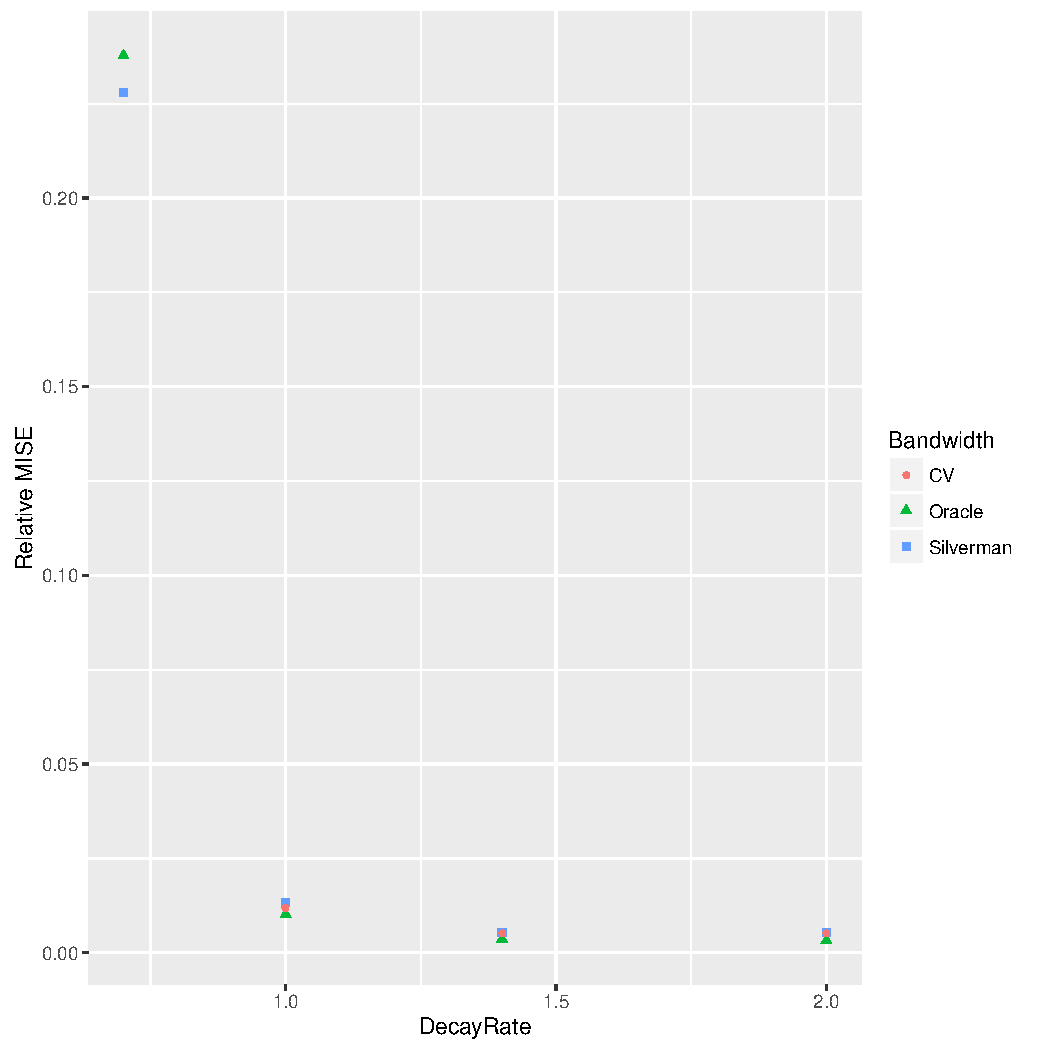
\includegraphics[width=\textwidth]{results/by_population_decay/RMISE-vs-population-decay}
    \caption{Relative MISE}
    \end{subfigure}
    \begin{subfigure}[b]{0.3\textwidth}
    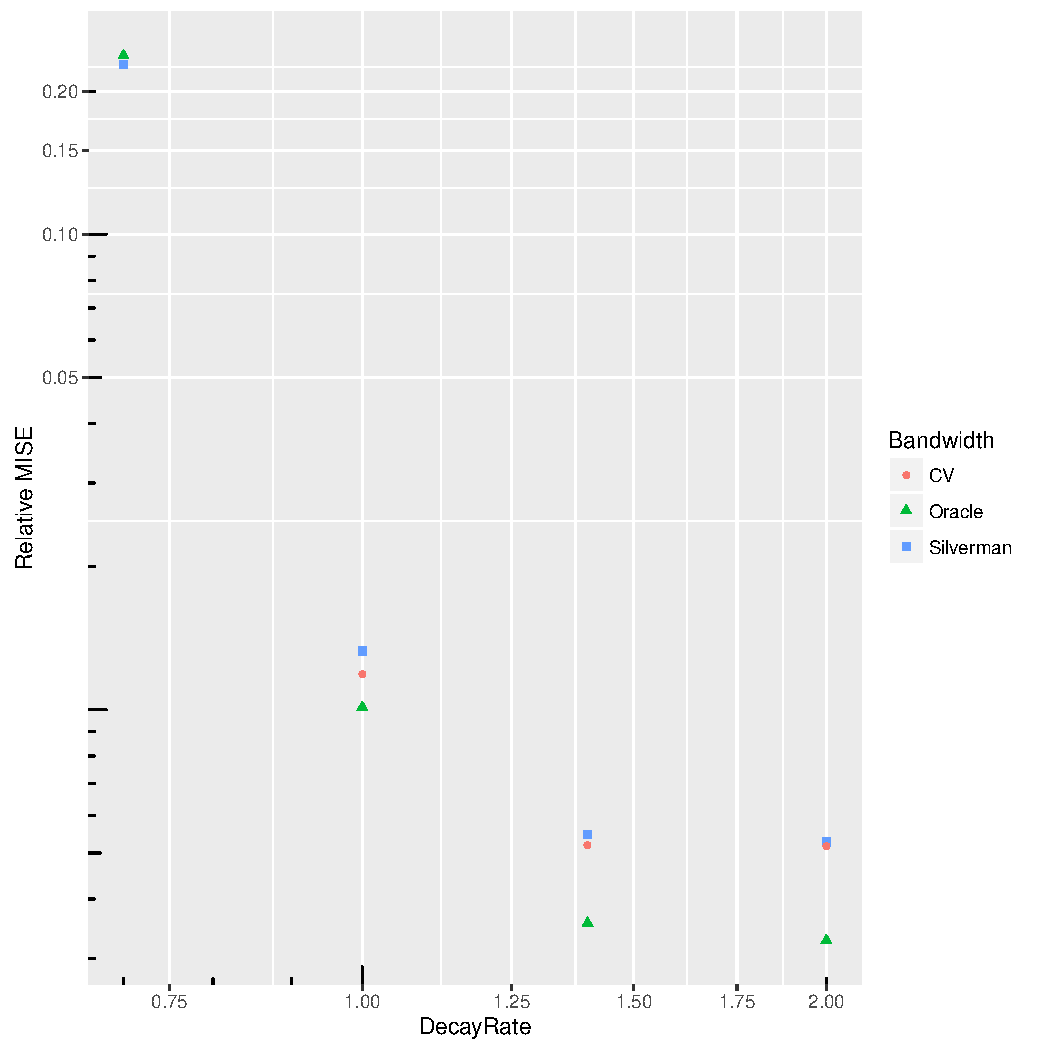
\includegraphics[width=\textwidth]{results/by_population_decay/RMISE-vs-population-decay-log-log}
    \caption{Relative MISE log-log}
    \end{subfigure}
    \caption[MISE: by risk decay]{Mean Integrated Squared Error vs. population decay rate}
    \label{fig:ise:pSD_100_1h}
\end{figure}


%%
%% Section
\section{Varying the distance between two peaks}
\label{sec:results:p1.4_100_G}

\begin{figure}[htbp]
    \centering
    \begin{subfigure}[b]{0.3\textwidth}
    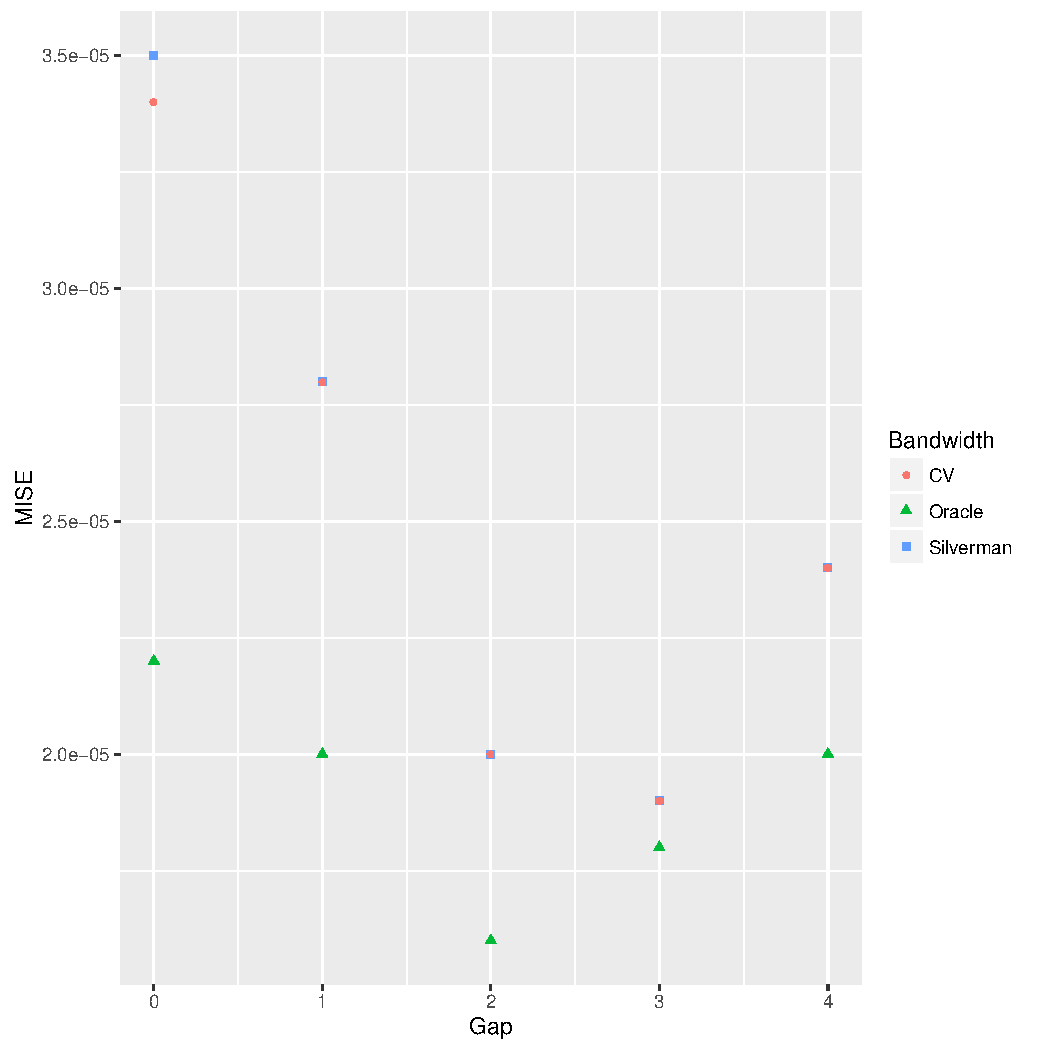
\includegraphics[width=\textwidth]{results/by_two_peaks/MISE-vs-risk-peak-gap}
    \caption{MISE}
    \end{subfigure}
    \begin{subfigure}[b]{0.3\textwidth}
    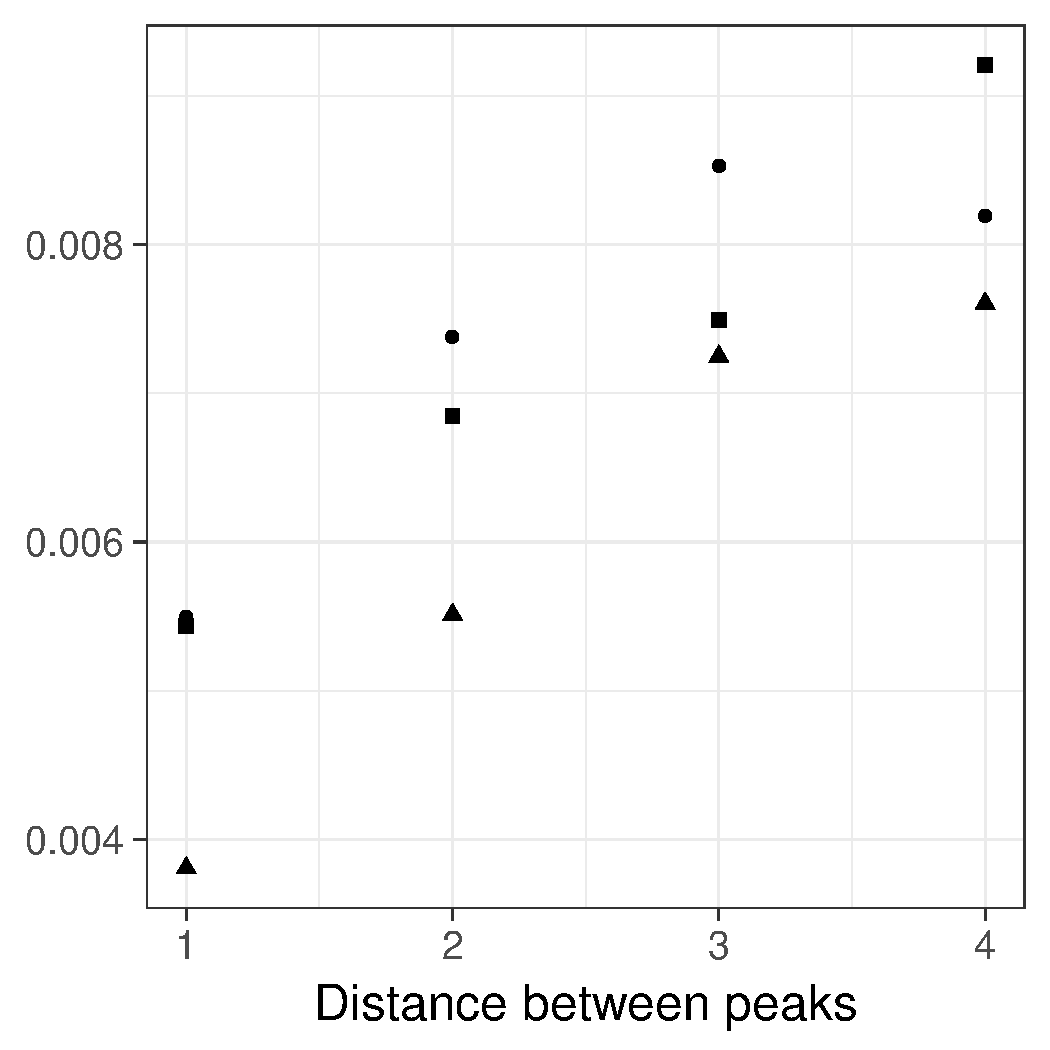
\includegraphics[width=\textwidth]{results/by_two_peaks/RMISE-vs-risk-peak-gap}
    \caption{Relative MISE}
    \end{subfigure}
    \begin{subfigure}[b]{0.3\textwidth}
    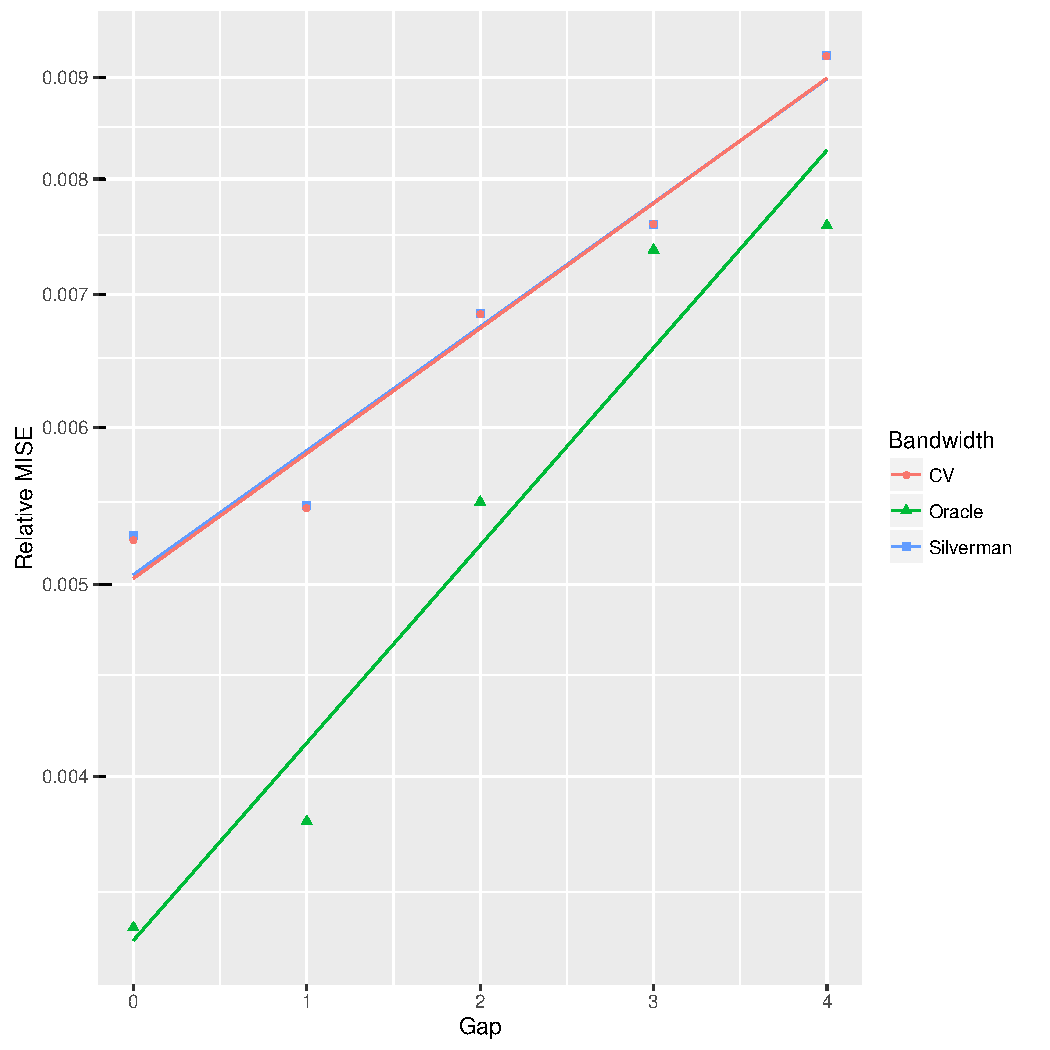
\includegraphics[width=\textwidth]{results/by_two_peaks/RMISE-vs-risk-peak-gap-log-log}
    \caption{Relative MISE log-log}
    \end{subfigure}
    \caption[MISE: by risk decay]{Mean Integrated Squared Error vs. distance between two risk peaks}
    \label{fig:ise:p1.4_100_G}
\end{figure}

%%
%% Section
\section{Varying the distance between the population and risk function peaks}
\label{sec:ise:p1.4_Gap_risk}

\begin{figure}[htbp]
    \centering
    \begin{subfigure}[b]{0.3\textwidth}
    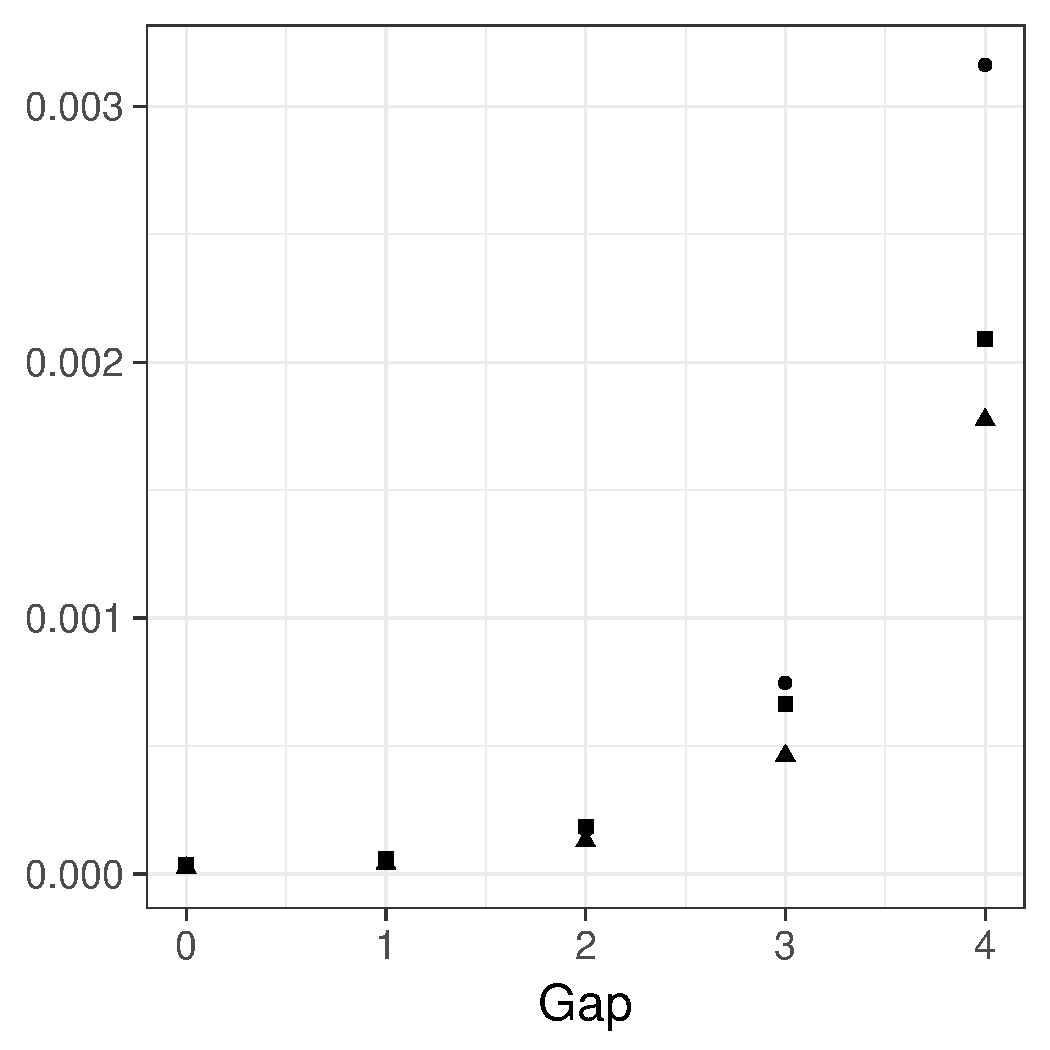
\includegraphics[width=\textwidth]{results/by_pop_risk_distance/MISE-vs-population-risk-gap}
    \caption{MISE}
    \end{subfigure}
    \begin{subfigure}[b]{0.3\textwidth}
    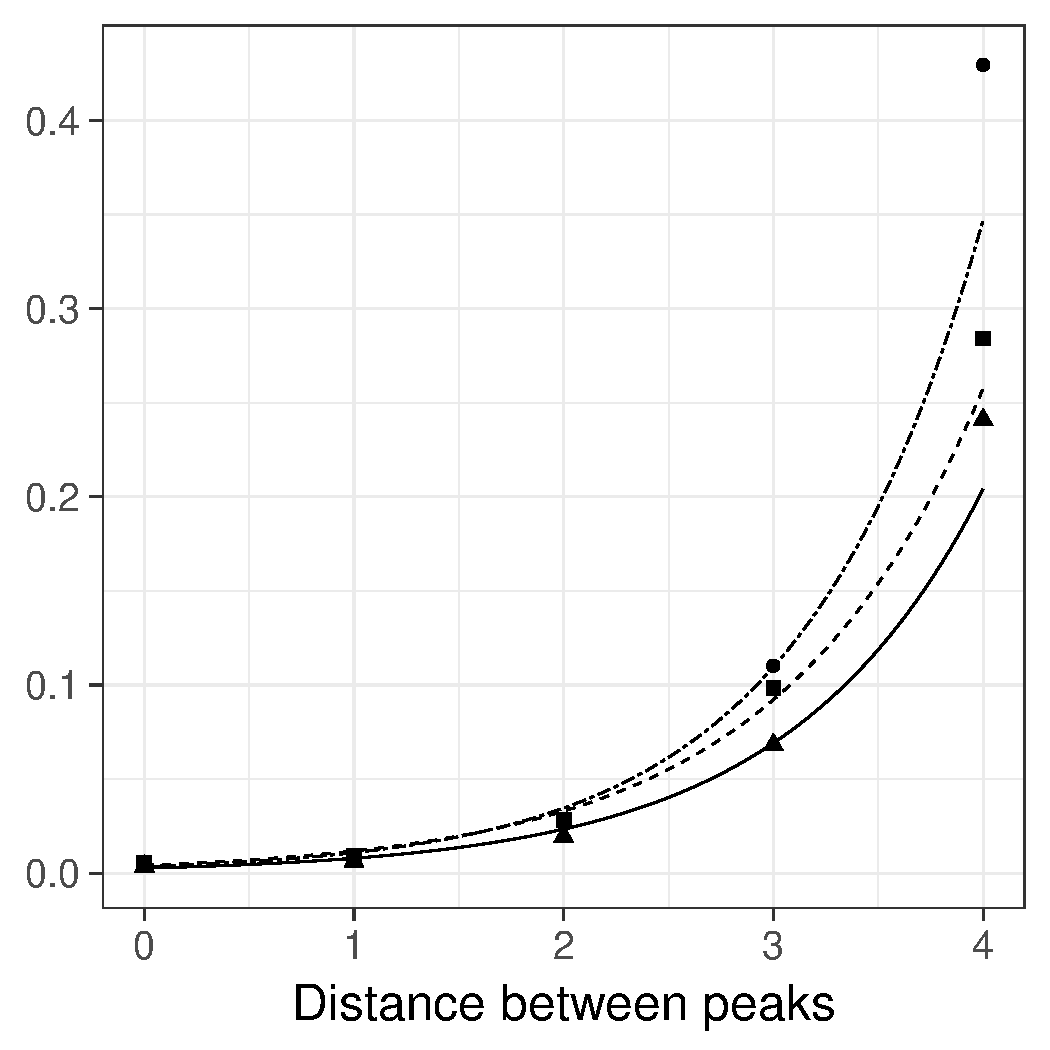
\includegraphics[width=\textwidth]{results/by_pop_risk_distance/RMISE-vs-population-risk-gap}
    \caption{Relative MISE}
    \end{subfigure}
    \begin{subfigure}[b]{0.3\textwidth}
    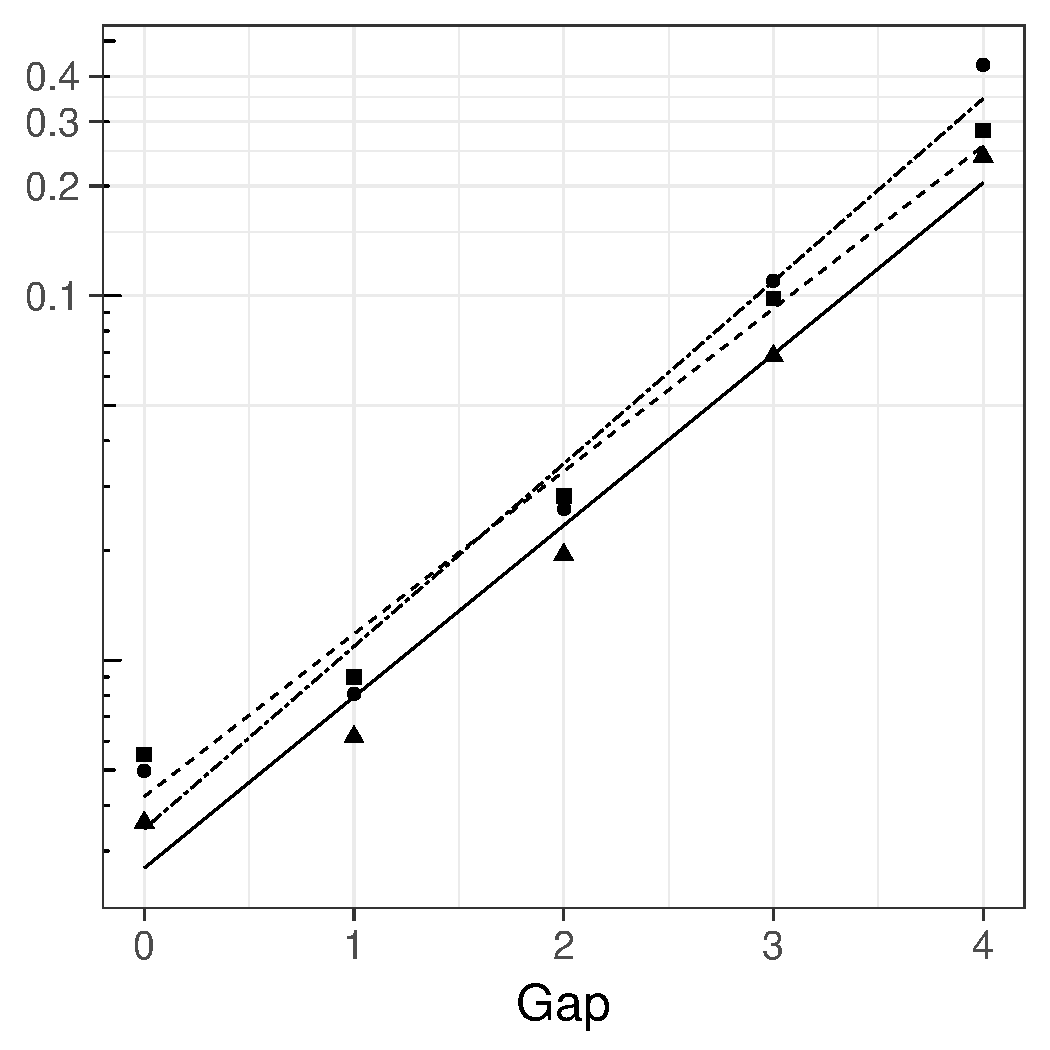
\includegraphics[width=\textwidth]{results/by_pop_risk_distance/RMISE-vs-population-risk-gap-log-log}
    \caption{Relative MISE log-log}
    \end{subfigure}
    \caption[MISE: by risk decay]{Mean Integrated Squared Error vs. distance between population and risk peaks}
    \label{fig:ise:p1.4_Gap_risk}
\end{figure}

